%%
%% This is file `example.tex',
%% generated with the docstrip utility.
%%
%% The original source files were:
%%
%% coppe.dtx  (with options: `example')
%% 
%% This is a sample monograph which illustrates the use of `coppe' document
%% class and `coppe-unsrt' BibTeX style.
%% 
%% \CheckSum{1416}
%% \CharacterTable
%%  {Upper-case    \A\B\C\D\E\F\G\H\I\J\K\L\M\N\O\P\Q\R\S\T\U\V\W\X\Y\Z
%%   Lower-case    \a\b\c\d\e\f\g\h\i\j\k\l\m\n\o\p\q\r\s\t\u\v\w\x\y\z
%%   Digits        \0\1\2\3\4\5\6\7\8\9
%%   Exclamation   \!     Double quote  \"     Hash (number) \#
%%   Dollar        \$     Percent       \%     Ampersand     \&
%%   Acute accent  \'     Left paren    \(     Right paren   \)
%%   Asterisk      \*     Plus          \+     Comma         \,
%%   Minus         \-     Point         \.     Solidus       \/
%%   Colon         \:     Semicolon     \;     Less than     \<
%%   Equals        \=     Greater than  \>     Question mark \?
%%   Commercial at \@     Left bracket  \[     Backslash     \\
%%   Right bracket \]     Circumflex    \^     Underscore    \_
%%   Grave accent  \`     Left brace    \{     Vertical bar  \|
%%   Right brace   \}     Tilde         \~}
%%

%% Adapted by Cabral, Felipe G. for undergraduated projects for POLI students

%% Adapted by Lima, Publio M. for undergraduated projects for EQ students

\documentclass[grad,numbers]{coppe}% Check the following table in order to know how to fill the command \documentclass[opt,numbers]{coppe} according to your degree, i.e., undergraduate projects, from POLI or EQ, master or doctor thesis from COPPE.

%% substitute where opt can be:
%% msc     - for Master Dissertations
%% dscexam - for Doctorade Qualification Exams
%% dsc     - for Doctorade Thesis
%% grad    - for Undergraduate Projects for Poli Students
%% gradeq  - for Undergraduate Projects for EQ Students

\usepackage{amsmath,amssymb}
\usepackage{hyperref}
\usepackage[utf8]{inputenc}
\usepackage[brazil]{babel}
\usepackage[T1]{fontenc}
\usepackage{graphicx}
\usepackage{array}
\usepackage{float}
\usepackage[center]{caption}
\usepackage{arydshln}
\usepackage{blkarray}
\usepackage{textcomp}
\usepackage{tikz}
\usepackage{svg}
\usepackage[normalem]{ulem}
\usetikzlibrary{automata,positioning}
\graphicspath{{figures/}}
\newtheorem{defi}{Definição}[chapter]
\newtheorem{obse}{Observação}[chapter]
\makelosymbols
\makeloabbreviations

\newcommand{\Inhib}{\textit{Inhib}}
\newcommand{\kernel}{\textit{kernel}}

%\includeonly{fundamentacao}

\begin{document}

\title{Diarização e Identificação de Locutor em Conteúdo de Vídeo Baseada em Análise de Expressão Facial via Aprendizado de Máquina Supervisionado}
\foreigntitle{Facial Expression Analysis for Speaker Diarization and Identification in Video Content via Supervised Machine Learning}
\author{Renan Fasolato}{Basilio}
\advisor{Prof.}{Geraldo Zimbrão}{da Silva}{D.Sc.}

\examiner{Prof.}{}{}
\examiner{Prof.}{}{}
\examiner{Prof.}{}{}

\department{ECI}

% Confira a tabela a seguir para saber como preencher o comando \department de acordo com seu curso (Graduação - Poli,Graduação - EQ) ou programa (Pós-Graduação - COPPE).


%%%%%% Para alunos da EQ %%%%%%

%% Course											Option
%% Engenharia Química                               EQ
%% Engenharia de Bioprocessos                       EB
%% Engenharia de Alimentos                          EAL
%% Química industrial                               QI

%%%%%% Para alunos da POLI %%%%%%

%% Course											Option
%% Engenharia Ambiental                             EA
%% Engenharia Civil                                 ECV
%% Engenharia de Computação e Informação            ECI
%% Engenharia de Controle e Automação               ECA
%% Engenharia de Materiais                          EMAT
%% Engenharia de Petróleo                           EPT
%% Engenharia de Produção                           EPR
%% Engenharia Eletrônica e de Computação            EEC
%% Engenharia Elétrica                              EET
%% Engenharia Mecânica                              EMC
%% Engenharia Metalúrgica                           EMET
%% Engenharia Naval e Oceânica                      ENO
%% Engenharia Nuclear                               ENU


%%%%%% Para alunos da COPPE %%%%%%

%% Program											Option
%% Engenharia Biomédica								PEB
%% Engenharia Civil									PEC
%% Engenharia Elétrica								PEE
%% Engenharia Mecânica								PEM
%% Engenharia Metalúrgica e de Materiais				PEMM
%% Engenharia Nuclear									PEN
%% Engenharia Oceânica								PENO
%% Planejamento Energético							PPE
%% Engenharia de Produção								PEP
%% Engenharia Química									PEQ
%% Engenharia de Sistemas e Computação				PESC
%% Engenharia de Transportes							PET

\date{\the\month}{\the\year}

\keyword{Aprendizado Supervisionado}
\keyword{Aprendizado de Máquina}
\keyword{Diarização de Locutor}

\maketitle
\frontmatter

\makecatalog

% TODO: Write Dedication
\dedication{To-Do: Write Dedication}

\tableofcontents

\mainmatter

\chapter{Introdução}
\label{chap:intro}

\section{Descrição do Problema}
\label{sec:desc}

A diarização de locutor consiste no processo de identificar os diferentes locutores em um conteúdo multimídia de forma a separa-los temporalmente, definindo quando quem falou, e produzir um tipo de roteiro para o mesmo.

Tradicionalmente, tenta-se resolver esse problema através da análise exclusiva do áudio, por meio da extração de \textit{features} na forma de vetores denominados \textit{I-vectors}\cite{zewoudieUseLongtermFeatures2018}, e subsequente clusterização destes.
Porém, trata-se de um problema difícil; o timbre, principal característica sonora responsável pela identificação do locutor pelo ser humano, é de caráter neurológico \cite{oxenhamPitchPerception2012}, produzido pela decomposição da onda sonora em seus harmônicos pelo trato auditivo.
E, ainda, como propriedade intrínseca da etapa de clusterização, a utilização desses algoritmos depende do conhecimento prévio do número de locutores que participam do áudio.

Dadas essas limitações, temos que o desempenho dos algoritmos considerados estado da arte é insuficiente, com taxa de erro de diarização (a partir daqui chamada de DER, do inglês \textit{Diarization Error Rate}) de cerca de 20\% nas bases tradicionais.
Portanto, a busca de outras técnicas capazes de prover um melhor desempenho nos leva a considerar também outros sinais constituintes do conteúdo multimídia, como o de vídeo do orador.

\section{Motivação}
\label{sec:motiv}

Em muitas situações, no processo de transcrição de áudio e vídeo, é interessante obter também a informação de quem está falando.
Com essa informação seria possível roteirizar a mídia, viabilizando um melhor entendimento e formatação do texto transcrito.
Além disso, essa informação adicional permite viabilizar novos critérios de busca sobre o texto transcrito, tornando possível filtrar os resultados por locutor.

\section{Definição do Problema}
\label{sec:problem-desc}

O problema de diarização de locutor consiste em particionar automaticamente um sinal de áudio tal que cada uma das partições geradas contenha as falas de um único locutor.
Trata-se de um problema muito relevante à área de reconhecimento de voz, já que entender quem falou em cada momento de uma gravação nos permite contextualizar diversos tópicos que dependem desse tipo de informação para sua legibilidade e interpretação, tais como a geração automática de transcrições de depoimentos judiciais e relatórios médicos eletrônicos.

A solução proposta neste trabalho consiste em construir um sistema capaz de diarizar as falas de um único locutor em tempo real a partir de um vídeo frontal do mesmo.
Para isso, o sistema de diarização deve ser capaz de, a partir de uma sequência de quadros extraída do vídeo original, determinar se o objeto da gravação está ou não falando. Neste trabalho iremos desconsiderar o áudio associado, já que o processamento deste foge à área de visão computacional.

Com esta finalidade, propomos uma arquitetura em três etapas:
\begin{enumerate}
    \item Com o uso de um identificador facial, o sistema identificará rostos nas imagens que lhe forem fornecidas. 
    \item Pontos de referência relevantes serão extraídos dos rostos identificados. 
    \item Através de um modelo de aprendizado de máquina previamente treinado, o sistema deverá ser capaz de determinar se o sujeito identificado está ou não falando.
\end{enumerate}

\section{Escopo}
\label{sec:scope}

De forma geral, gostaríamos de identificar as falas de todos os oradores do texto.
No entanto, muitas vezes é suficiente identificar apenas um destes, por exemplo no caso de audiências e depoimentos do Tribunal de Justiça.
Nesse caso específico desejamos identificar com maior precisão os trechos falados pelo depoente, independentemente do número de participantes da audiência, de forma a distinguir futuramente o que foi dito pelo mesmo em seu depoimento.

Para esta finalidade, assumimos que esteja disponível um vídeo frontal da face do locutor (depoente), além do áudio combinado de todos os participantes, em canal monoaural.
Esta suposição é feita tendo em vista as características dos dados reais, tendo o conhecimento de que caso o áudio estivesse separado em canais correspondentes a cada locutor o problema se tornaria trivial.
Assim, este trabalho ficará limitado a tratar de casos nos quais estas informações estejam disponíveis, e com a determinação de que o vídeo deve ser de boa qualidade.

\section{Estrutura do Trabalho}
\label{sec:structure}

Este trabalho se encontra organizado da seguinte maneira:

No capítulo 2 apresentamos a fundamentação teórica referente às técnicas e tecnologias utilizadas na implementação de cada uma das etapas propostas nesse trabalho.
Em primeiro momento, fazemos uma revisão das abordagens e implementações formuladas para resolução do problema de alinhamento facial até hoje. 
Em seguida, apresentamos os conceitos e técnicas críticas para nossa implementação, sendo estas as redes neurais convolucionais, detecção de objetos por histograma de gradientes orientados, e alinhamento facial.

No capítulo 3 apresentamos a nossa implementação do sistema proposto. 
Abordamos tópicos como as ferramentas utilizadas, pré-processamento dos dados de treinamento, e a arquitetura proposta para a rede neural convolucional.
Por fim, discutimos a implementação da aplicação final, para lidar com dados não tratados previamente.

No capítulo 4 demonstramos os resultados de nosso método quando aplicado sobre dataset fornecido pela Defensoria Pública do Estado do Rio de Janeiro, que contém vídeos dos participantes individuais\sout{, em alta resolução e} com as características desejadas.

Por fim, no capítulo 5, resumimos e apresentamos nossas conclusões quanto ao trabalho realizado, discutindo os resultados obtidos e os fatores que contribuíram para estes, e enumeramos trabalhos futuros a serem realizados sobre o mesmo tema.

No apêndice, apresentamos o código fonte desenvolvido para este trabalho.
\chapter{Revisão Bibliográfica}

\section{Trabalhos Correlatos}
\label{sec:related-work}

O problema de diarização de locutor é historicamente abordado de duas maneiras distintas.
A abordagem tradicional envolve a extração de vetores de características do áudio que se deseja diarizar, podendo ser estes \textit{I-Vectors} \cite{dehakFrontEndFactorAnalysis2011}, extraídos por meio de transformações matriciais aplicadas sobre o sinal, ou \textit{X-Vectors} \cite{snyderXVectorsRobustDNN2018}, obtidos através do uso de redes neurais profundas.
A partir de então, estes vetores podem ser clusterizados \cite{sellSpeakerDiarizationPlda2014} quando informações referentes ao número de locutores é conhecido, ou, mais recentemente, utilizados como entrada de uma rede neural LSTM \cite{wangSpeakerDiarizationLSTM2018}.

No entanto, a introdução das redes neurais convolucionais para reconhecimento de ações humanas em sinais de vídeos \cite{ji3DConvolutionalNeural2013, karpathyLargeScaleVideoClassification2014} implicou na concepção de uma nova abordagem.
Nesta, com o objetivo de melhorar a diarização de sinais heterogêneos, é utilizado um algoritmo de reconhecimento de ações também sobre o sinal de vídeo \cite{hersheyAudiovisualGraphicalModels2004}, que se supõe estar sincronizado ao áudio correspondente.
O reconhecimento de ações é, nesse caso, utilizado para identificar a fala do locutor e, quando combinado com os sinais de áudio, é capaz de produzir resultados melhores do que o estado da arte no processamento exclusivo de áudio \cite{ephratLookingListenCocktail2018}.

\section{Fundamentação Teórica}

Nesta seção discutiremos a fundamentação teórica das várias tecnologias utilizadas na execução do trabalho. Primeiramente, na seção \ref{sec:ann}, apresentaremos o conceito de redes neurais artificiais, utilizadas para construção do identificador de fala. Depois, na seção \ref{sec:facialrecog}, discutiremos a técnica de \textit{histograma de gradientes orientados}, utilizada pelo identificador frontal de rostos. Por fim, na seção \ref{sec:faciallm}, apresentaremos o conceito de floresta de regressão, utilizado para a detecção de marcadores faciais.

\subsection{Redes Neurais Artificiais}
\label{sec:ann}

Redes Neurais Artificiais são um conjunto de algoritmos inspirados pelo funcionamento do cérebro humano, introduzidos pela primeira vez em 1943 quando Warren McCulloch e Walter Pitts modelaram o funcionamento de neurônios através de circuitos elétricos simples\cite{mccullochLogicalCalculusIdeas1943}. 
Esse modelo continuou evoluindo ao longo dos anos, culminando no desenvolvimento do \textit{Perceptron} por Rosenblatt em 1958 \cite{rosenblattPerceptronProbabilisticModel1958} (figura \ref{fig:perceptron}), um algoritmo de classificação binária semelhante a uma rede neural composta por um único neurônio.

No entanto, devido à falta de capacidade computacional e ao grande volume de dados necessários para o treinamento de redes neurais, estes algoritmos permaneceram apenas um conceito acadêmico durante vários anos.
Somente em 2006, Geoffrey Hinton proporia formalmente o conceito de rede neural profunda \cite{hintonFastLearningAlgorithm2006}, um tipo de rede neural composto por múltiplas camadas de neurônios totalmente conectadas.

\begin{figure}[ht]
    \centering
    \begin{tikzpicture}[]
    \node[coordinate] (input) [] {};
    \node[state, circle, align=center] (input1) at (input) [] {$x_2$};
    \node[state, circle, align=center] (input2) [above=of input1, yshift=-0.3cm] {$x_1$};
    \node[state, circle, align=center] (input3) [below=of input1, yshift=0.3cm] {$x_3$};
    \node[draw=none, fill=none] [below=of input3, yshift=-0.3cm] (inputs_label) {Entrada};

    \node[coordinate] (hidden1) [right=of input, xshift=1.5cm] {};
    \node[state, circle, align=center] (hidden11) at (hidden1) [] {};
        \draw [->, color=gray] (input1) -- (hidden11);
        \draw [->, color=gray] (input2) -- (hidden11);
        \draw [->, color=gray] (input3) -- (hidden11);
    \node[state, circle, align=center] (hidden12) [above=of hidden11, yshift=-0.7cm] {};
        \draw [->, color=gray] (input1) -- (hidden12);
        \draw [->, color=gray] (input2) -- (hidden12);
        \draw [->, color=gray] (input3) -- (hidden12);
    \node[state, circle, align=center] (hidden13) [above=of hidden12, yshift=-0.7cm] {};
        \draw [->, color=gray] (input1) -- (hidden13);
        \draw [->, color=gray] (input2) -- (hidden13);
        \draw [->, color=gray] (input3) -- (hidden13);
    \node[state, circle, align=center] (hidden14) [below=of hidden11, yshift=0.7cm] {};
        \draw [->, color=gray] (input1) -- (hidden14);
        \draw [->, color=gray] (input2) -- (hidden14);
        \draw [->, color=gray] (input3) -- (hidden14);
    \node[state, circle, align=center] (hidden15) [below=of hidden14, yshift=0.7cm] {};
        \draw [->, color=gray] (input1) -- (hidden15);
        \draw [->, color=gray] (input2) -- (hidden15);
        \draw [->, color=gray] (input3) -- (hidden15);

    \node[coordinate] (hidden2) [right=of hidden1, xshift=1.5cm] {};
    \node[state, circle, align=center] (hidden21) [above=of hidden2, yshift=-0.7cm] {};
        \draw [->, color=gray] (hidden11) -- (hidden21);
        \draw [->, color=gray] (hidden12) -- (hidden21);
        \draw [->, color=gray] (hidden13) -- (hidden21);
        \draw [->, color=gray] (hidden14) -- (hidden21);
        \draw [->, color=gray] (hidden15) -- (hidden21);
    \node[state, circle, align=center] (hidden22) [above=of hidden21, yshift=-0.7cm] {};
        \draw [->, color=gray] (hidden11) -- (hidden22);
        \draw [->, color=gray] (hidden12) -- (hidden22);
        \draw [->, color=gray] (hidden13) -- (hidden22);
        \draw [->, color=gray] (hidden14) -- (hidden22);
        \draw [->, color=gray] (hidden15) -- (hidden22);
    \node[state, circle, align=center] (hidden23) [below=of hidden2, yshift=0.7cm] {};
        \draw [->, color=gray] (hidden11) -- (hidden23);
        \draw [->, color=gray] (hidden12) -- (hidden23);
        \draw [->, color=gray] (hidden13) -- (hidden23);
        \draw [->, color=gray] (hidden14) -- (hidden23);
        \draw [->, color=gray] (hidden15) -- (hidden23);
    \node[state, circle, align=center] (hidden24) [below=of hidden23, yshift=0.7cm] {};
        \draw [->, color=gray] (hidden11) -- (hidden24);
        \draw [->, color=gray] (hidden12) -- (hidden24);
        \draw [->, color=gray] (hidden13) -- (hidden24);
        \draw [->, color=gray] (hidden14) -- (hidden24);
        \draw [->, color=gray] (hidden15) -- (hidden24);
    \node[draw=none, fill=none] [right=of inputs_label, xshift=0.25cm] (hidden_label) {Camadas Ocultas};

    \node[coordinate] (output) [right=of hidden2, xshift=1.5cm] {};
    \node[state, circle, align=center] (output1) [above=of output, yshift=-0.75cm] {$y_1$};
        \draw [->, color=gray] (hidden21) -- (output1);
        \draw [->, color=gray] (hidden22) -- (output1);
        \draw [->, color=gray] (hidden23) -- (output1);
        \draw [->, color=gray] (hidden24) -- (output1);
    \node[state, circle, align=center] (output2) [below=of output, yshift=0.75cm] {$y_2$};
        \draw [->, color=gray] (hidden21) -- (output2);
        \draw [->, color=gray] (hidden22) -- (output2);
        \draw [->, color=gray] (hidden23) -- (output2);
        \draw [->, color=gray] (hidden24) -- (output2);
    \node[draw=none, fill=none] [right=of hidden_label, xshift=0.25cm] (output_label) {Saída};

\end{tikzpicture}
    \caption{Ilustração de uma rede neural profunda com 3 camadas.}
    \label{fig:dnn}
\end{figure}

Recentemente, com o desenvolvimento de algoritmos para o treinamento de redes neurais em GPU (do Inglês \textit{Graphics Processing Unit}), que possibilitaram o treinamento mais rápido e eficiente de redes neurais de múltiplas camadas, assim como o crescente volume de dados disponível para treinamento, o tópico de redes neurais vem rapidamente ganhando popularidade.
Algoritmos desse tipo já são utilizados em diversas áreas da ciência, incluindo aplicações em medicina \cite{hannunCardiologistLevelArrhythmiaDetection2019,phamPredictingHealthcareTrajectories2017,houDeepSFDeepConvolutional2018}, previsão do tempo \cite{akramSequenceSequenceWeather2016}, veículos autônomos \cite{bojarskiEndEndLearning2016,peddagollaLaneDetectionAutonomous}, entre outras \cite{abiodunStateoftheartArtificialNeural2018}.

Tratam-se de algoritmos próprios para problemas que envolvem o reconhecimento de padrões, e a capacidade de treina-los a partir de dados existentes os torna eficazes para aplicação em tópicos nos quais as relações entre os dados de entrada não sejam totalmente conhecidas.

\subsubsection{Neurônios Artificiais}

Biologicamente, quando o potencial elétrico na base do axônio de um neurônio chega a um valor pré-determinado, por meio do acúmulo de sinais de entrada recebidos pelos dendritos, um pulso elétrico é gerado e propagado até as sinapses, terminais nos quais o neurônio conecta com os demais.
Trata-se de um sinal binário; o neurônio pode ou não estar ativado a cada instante. No entanto, a frequência relativa das ativações pode conter informação \cite{behnkeHierarchicalNeuralNetworks2003}.

\begin{figure}[H]
    \centering
    \includesvg[width=0.7\textwidth]{neurono-ido.svg}
    \caption{A estrutura de um neurônio biológico. Imagem adaptada de \cite{dhp1080IdoSkemoPri2016}.}
    \label{fig:bio_neuron}
\end{figure}

Funções de Ativação, também conhecidas como funções de propagação ou neurônios artificiais quando aplicadas no contexto de redes neurais, buscam modelar de forma simplificada esses aspectos biológicos.
Elas recebem como entrada os valores resultantes das camadas anteriores, ponderados por pesos específicos a cada conexão, e, quando estes valores atingem um limiar de excitação pré-determinado, os transformam em uma única saída.

\begin{figure}[H]
    \centering
    \begin{tikzpicture}
    \node[state, circle, align=center] (activation) [] {$\phi(x)$};
    
    \node[state, circle, align=center] (sum) [left=of activation] {$\sum$};
        \draw [->] (sum) -- (activation);
        
    \node[state, circle, align=center] (input1) [above left=of sum, yshift=-1cm, xshift=-1cm] {$x_2$};
        \draw [->] (input1) -- node [midway, above] {$w_2$} (sum);
        
    \node[state, circle, align=center] (input0) [above=of input1, yshift=-0.5cm] {$x_1$};
        \draw [->] (input0) -- node [midway, above] {$w_1$} (sum);
        
    \node[state, circle, align=center] (input2) [below left=of sum, yshift=1cm, xshift=-1cm] {$x_3$};
        \draw [->] (input2) -- node [midway, above] {$w_3$} (sum);
        
    \node[state, circle, align=center] (input3) [below=of input2, yshift=-0.5cm] {$x_n$};
        \path (input2) -- (input3) node [font=\Huge, midway, sloped] {$\dots$};
        \draw [->] (input3) -- node [midway, above=0.5em] {$w_n$} (sum);
        
    \node[draw=none, fill=none] [right=of activation] (output) {Saída};
        \draw [->] (activation) -- (output);
        
    \node[draw=none, fill=none] [below=of input3, yshift=0.7cm] (inputs) {Entradas};

\end{tikzpicture}
    \caption{O \textit{Perceptron}, uma rede neural com um único neurônio.}
    \label{fig:perceptron}
\end{figure}

Geralmente, a função de ativação é constante e independente do processo de treinamento da rede neural; o ajuste é feito sobre os pesos das conexões, através algoritmo de retropropagação \cite{dreyfusArtificialNeuralNetworks1990}.
O algoritmo é capaz de, a partir do resultado de uma camada, calcular o efeito de cada peso sobre o gradiente da função.
Assim, ele possibilita a utilização de algoritmos tradicionais de otimização para encontrar os pesos locais de cada conexão, mesmo em redes com múltiplas camadas de centenas de neurônios, em função do efeito global destes.

Comumente, são utilizadas como função de ativação as funções ReLU (\textit{Rectified Linear Unit}), tangente hiperbólica, sigmoide, e Heaviside, em função do intervalo de saída e comportamento desejado.

\begin{equation}\label{eq:relu}
    \phi(x) = \left\{
        \begin{array}{ll}
            0, & x \le 0\\
            x, & x > 0
        \end{array}
    \right.
\end{equation}

A função ReLU (equação \ref{eq:relu}), utilizada neste trabalho, tem comportamento tal que sua ativação ocorre sempre que $x>0$, com o valor resultante sendo o próprio valor de $x$. 
Essa função é ideal para aplicações em redes neurais profundas pois o gradiente é preservado após cada camada da rede, o que não ocorre com as funções sigmoide e tangente hiperbólica.
Nessas, o gradiente tende a valores infinitesimalmente pequenos após camadas sucessivas, dificultando o uso do algoritmo de retropropagação.
Além disso, o treinamento de redes neurais profundas que utilizam a função ReLU é mais rápido do que o das outras funções de ativação, devido à sua simplicidade \cite{krizhevskyImageNetClassificationDeep2017}.

\subsubsection{Redes Neurais Convolucionais}
\label{sec:convnet}

Redes Neurais Convolucionais são redes neurais compostas por uma ou mais camadas de convolução.
São ideais para o tratamento de dados matriciais, como por exemplo imagens, que constituem em uma matriz bi-dimensional de pixels, ou vídeos, matrizes tridimensionais de imagens.
Essas redes são capazes de identificar relações entre os elementos adjacentes de uma matriz, e, através da técnica de Max Pooling, focar somente nos pontos mais relevantes, mesmo em conjuntos de dados muito grandes.

\paragraph{Convolução e Filtros}
\label{sec:convolution}

A convolução é uma técnica matemática que consiste na aplicação de uma matriz, denominada matriz de convolução ou \textit{filtro} quando utilizada no contexto de processamento de imagens, sobre cada elemento de uma outra matriz.
Esse processo produz uma nova matriz na qual o valor de cada elemento corresponde ao seu valor e o valor de seus vizinhos, ponderados pelos valores da matriz de convolução, denominados \kernel\ da convolução.

Para dados bi-dimensionais, a operação de convolução pode ser descrita da seguinte forma:

\begin{equation}
    g(x,y) = \omega * f(x,y) = \sum\limits_{s=-a}^a\sum\limits_{t=-b}^b\omega(s,t)f(x-s, y-t)
\end{equation}

Essa técnica é frequentemente utilizada em áreas que trabalham com imagens, como na área de veículos autônomos, onde é capaz de identificar as faixas pintadas sobre o asfalto \cite{peddagollaLaneDetectionAutonomous}, assim como outros veículos e pedestres na rua.
Com a aplicação dessa, é possível remover características da imagem de entrada irrelevantes para o problema que se deseja resolver, como mostra a figura \ref{fig:conv}, diminuindo a complexidade do problema a cada camada.

\begin{figure}[ht]
    \centering
    \begin{tikzpicture}
    \node[inner sep=0pt] (pre_conv)
        {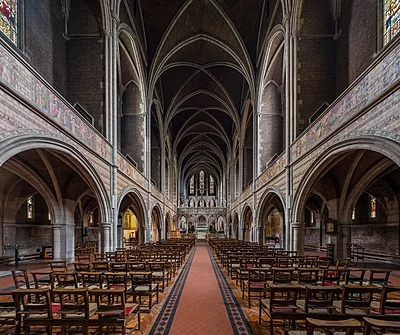
\includegraphics[width=0.3\textwidth]{photo_conv_1.png}};
    \node[state, rectangle, align=center] (kernel) [right=of pre_conv] 
        {
            $
                \begin{bmatrix}
                    0 & -1 & 1 \\
                    0 & -1 & 1 \\
                    0 & -1 & 1
                \end{bmatrix}
            $\\
            \textit{Kernel}
        };
        \draw [->] (pre_conv) -- (kernel);
    \node[inner sep=0pt] (post_conv) [right=of kernel]
        {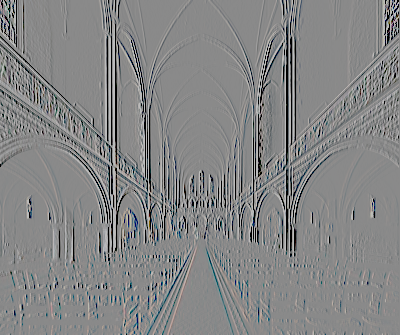
\includegraphics[width=0.3\textwidth]{photo_conv_2.png}};
        \draw [->] (kernel) -- (post_conv);
\end{tikzpicture}
    \caption{O resultado da aplicação de um \kernel\ simples para detecção de bordas verticais a uma foto. 
    O \kernel\ é aplicado a cada pixel da imagem, substituindo o valor deste pela soma de sua vizinhança ponderada pelos valores da matriz. 
    Foto original obtida de \cite{diliffEnglishLookingEast2015}.}
    \label{fig:conv}
\end{figure}

No contexto de redes neurais convolucionais, isso consiste em neurônios que realizam uma operação de convolução sobre os dados de entrada.
O \kernel\ da matriz de convolução é treinado de forma a identificar os aspectos da entrada mais relevantes para o problema, através do algoritmo de retropropagação.

\paragraph{Pooling}
\label{sec:pooling}

Um outro tipo de camada tradicional nas redes neurais convolucionais é a camada de \textit{pooling}, ou ``agrupamento''.
Esse tipo de camada tem como função reduzir o número e complexidade dos dados de entrada e promover uma melhor generalização dos dados espaciais.
Isso é necessários pois as camadas convolucionais tendem a manter a localização espacial das características detectadas na matriz de entrada, informação que na maioria dos casos não é relevante para o problema que se deseja resolver.

A operação consiste em subdividir a matriz de entrada em conjuntos de valores e, segundo um critério especificado, escolher entre estes um único valor resultante.

\begin{figure}[ht]
    \centering
    \begin{tikzpicture}
    \filldraw[fill=red!20!white] (-1, 1) rectangle (0, 0);
    \filldraw[fill=green!20!white] (0, 1) rectangle (1, 0);
    \filldraw[fill=blue!20!white] (-1, -1) rectangle (0, 0);
    \filldraw[fill=yellow!20!white] (0, 0) rectangle (1, -1);
    \draw[step=0.5cm, color=gray] (-1, -1) grid (1, 1);
    \node[coordinate] (pre_pool) at (1, 0) {};
    \node at (-0.75, +0.75) {1};
    \node at (-0.25, +0.75) {2};
    \node at (+0.25, +0.75) {7};
    \node at (+0.75, +0.75) {5};
    \node at (-0.75, +0.25) {4};
    \node at (-0.25, +0.25) {3};
    \node at (+0.25, +0.25) {0};
    \node at (+0.75, +0.25) {9};
    \node at (-0.75, -0.25) {7};
    \node at (-0.25, -0.25) {0};
    \node at (+0.25, -0.25) {6};
    \node at (+0.75, -0.25) {1};
    \node at (-0.75, -0.75) {3};
    \node at (-0.25, -0.75) {4};
    \node at (+0.25, -0.75) {2};
    \node at (+0.75, -0.75) {8};

    \filldraw[fill=red!20!white] (4, 0.5) rectangle (4.5, 0);
    \filldraw[fill=green!20!white] (4.5, 0.5) rectangle (5, 0);
    \filldraw[fill=blue!20!white] (4, 0) rectangle (4.5, -0.5);
    \filldraw[fill=yellow!20!white] (4.5, 0) rectangle (5, -0.5);
    \draw[step=0.5cm, color=gray] (4-0.001, -0.5) grid (5, 0.5);
    \node[coordinate] (post_pool) at (4, 0) {};
    \node at (4.25, +0.25) {4};
    \node at (4.25, -0.25) {7};
    \node at (4.75, +0.25) {9};
    \node at (4.75, -0.25) {8};

    \draw[->] (pre_pool) -- (post_pool);
    \path [] (pre_pool) -- node [midway, above] {Max Pooling} node [midway, below] {$2\times2$} (post_pool);
\end{tikzpicture}
    \caption{O resultado da operação de \textit{Max Pooling} com dimensão $2\times2$ sobre uma matriz de entrada.}
    \label{fig:maxpool}
\end{figure}

No contexto de redes neurais convolucionais, no entanto, dado que os valores resultantes da camada convolucional teriam sido filtrados por uma função de ativação não-linear, como a ReLU (equação \ref{eq:relu}), temos que os valores obtidos correspondem à intensidade da ativação dos neurônios.
Assim, devido ao fato de que valores maiores devem corresponder a características de maior importância na matriz de entrada, temos dois critérios mais usados para a operação:

\begin{description}
    \itemsep0em 
    \item \textit{\textbf{Max Pooling}}: Para cada grupo, calcula o valor máximo (figura \ref{fig:maxpool}).
    \item \textit{\textbf{Average Pooling}}: Para cada grupo, calcula a média dos valores.
\end{description}

A escolha entre esses critérios é feita em função do propósito da camada anterior; se esta for, por exemplo, um detector de bordas em imagens, temos que a técnica de \textit{Max Pooling} será preferível, visto que as bordas serão sempre o maior valor do grupo, enquanto os demais elementos terão valor zero.
Já no caso de se tratar de um reconhecedor de variação temporal, a técnica de \textit{Average Pooling} pode ser preferível, já que será capaz de manter informações sobre o valor médio dos elementos no instante que está sendo comprimido.

\subsection{Histograma de Gradientes Orientados}
\label{sec:facialrecog}

Histograma de Gradientes Orientados ou HOG, do inglês \textit{Histogram of Oriented Gradients}, é uma técnica de visão computacional utilizada para detecção de objetos em imagens, introduzida pela primeira vez em 1982 por Robert McConnel \cite{mcconnellMethodApparatusPattern1986}, e formalizada em 1994 por Freeman e Roth \cite{freemanOrientationHistogramsHand}.
Trata-se do treinamento de um histograma de blocos descritivos dos gradientes que se espera observar em cada um dos pontos que se deseja conhecer, e posterior comparação deste com os gradientes de áreas ou células da imagem de entrada.

% NOTE: Reescrever? "Uma dessas técnicas é a F-HOG \cite{felzenszwalbObjectDetectionDiscriminatively}..."
\{Devo falar isso assim?\} A implementação de Histograma de Gradientes Orientados aqui discutida é aquela adotada pela biblioteca Dlib (seção \ref{subsec:dlib}), a F-HOG, baseada no artigo de Pedro F. Felzenszwalb, \textit{et al}. \cite{felzenszwalbObjectDetectionDiscriminatively}.

\begin{figure}[ht]
    \centering
    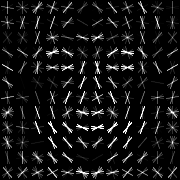
\includegraphics[width=0.30\textwidth]{face_fhog_filters.png}
    \caption{Um exemplo de detector HOG para identificação facial frontal. Imagem retirada de \cite{kingDlib18Released}.}
    \label{fig:dlib_hog}
\end{figure}

A técnica consiste em, primeiramente, calcular os gradientes de cada ponto da imagem, normalizada quanto à cor através de sua conversão a escala de cinza, a partir da aplicação de um vetor de diferenciação $[-1, 0, +1]$ e seu transposto a cada pixel desta.
Esse processo calcula um ângulo $\theta$ e intensidade $r$, representando o gradiente local de cada um dos pontos aos quais é aplicado.
Os gradiente são, então, discretizados para uma de 18 direções pré-definidas.

Uma vez calculados os gradientes em todos os pontos da figura, estes são agrupados em regiões espaciais densas e retangulares, passando a compor as células do histograma, no processo chamado de ``agrupamento espacial'' (\textit{spatial/orientation binning}).
A orientação final de cada bloco é, então, calculada a partir dos gradientes da região espacial que integram, através da soma de suas orientações.
Isso garante a invariância do reconhecedor a pequenas alterações nas bordas, além de diminuir o tamanho deste, já que em geral o valor resultante das células tenderá ao mesmo valor quando agrupadas.

\begin{equation}\label{eq:hog_energy}
    \begin{split}
        N_{\delta,\gamma}(i,j) = & \left(
            \left\Vert C(i,j) \right\Vert ^2 +
            \left\Vert C(i+\delta,j) \right\Vert ^2 +
            \right.\\ 
            & + \left. \left\Vert C(i,j+\gamma) \right\Vert ^2 +
            \left\Vert C(i+\delta,j+\gamma) \right\Vert ^2
            \right)^{1/2}, \qquad \delta,\gamma \in \{-1, 1\}
    \end{split}
\end{equation}

\begin{equation}\label{eq:hog_norm}
    H(i,j) = \left(\begin{matrix}
        T_\alpha(C(i,j)/N_{-1,-1}(i, j))\\
        T_\alpha(C(i,j)/N_{+1,-1}(i, j))\\
        T_\alpha(C(i,j)/N_{+1,+1}(i, j))\\
        T_\alpha(C(i,j)/N_{-1,+1}(i, j))
    \end{matrix}\right)
\end{equation}

É feita, então, a normalização dos blocos descritores. 
Primeiramente, é calculada a energia de cada bloco de 4 células do histograma, segundo a equação \ref{eq:hog_energy}. 
Depois, o valor de cada uma delas é normalizado em relação a sua vizinhança, e cada um de seus componentes é truncado em relação a um fator de truncamento $\alpha = 0.2$, através da equação \ref{eq:hog_norm}.

% TODO: Continue writing this section.

\subsection{Detecção de Marcadores Faciais}
\label{sec:faciallm}
\chapter{Implementação}
\label{chap:impl}

Neste capítulo discutiremos tópicos relacionados à implementação do sistema de diarização de locutor proposto. 

Na seção \ref{sec:tools} apresentamos as ferramentas principais utilizadas no desenvolvimento deste trabalho.
Em seguida, na seção \ref{sec:preproc}, apresentamos o trabalho realizado para preparação e pré-processamento dos dados.

Foram desenvolvidos dois conjuntos scripts distintos para este trabalho; um sistema para treinamento da rede neural convolucional, e outro para a diarização de locutor em um vídeo com as características definidas anteriormente.
Sendo assim, discutiremos a arquitetura utilizada para treinamento do modelo na seção \ref{sec:train}, e a utilizada no processamento de uma mídia de entrada na seção \ref{sec:application}.

\section{Ferramentas}
\label{sec:tools}

Nesta seção apresentamos as principais ferramentas utilizadas durante a implementação deste trabalho.
Definiremos suas principais características, assim como as funcionalidades das mesmas que foram utilizadas, e as motivações por trás de sua escolha.

Na seção \ref{subsec:dlib} apresentaremos a biblioteca Dlib, utilizada para propósito de identificação e demarcação facial no projeto.
Em seguida, na seção \ref{subsec:tf} apresentaremos a biblioteca Tensorflow, utilizada por sua robusta implementação do modelo de rede neural convolucional.
Na seção \ref{subsec:environ} apresentaremos o ambiente utilizado para treinamento do modelo, assim como seus recursos computacionais.
Por fim, na seção \ref{subsec:otools}, mencionaremos brevemente as demais ferramentas utilizadas em caráter pontual no trabalho, e que, por essa razão, não receberam seções dedicadas.

\subsection{Dlib}
\label{subsec:dlib}
A Dlib\cite{dlib09} é uma biblioteca de código aberto desenvolvida em C++ e com interface em Python.
Trata-se de uma biblioteca generalista, contendo implementações de algoritmos para processamento paralelo, grafos, entre outros.
Porém, seu foco principal se encontra nas áreas de aprendizado de máquina, processamento de imagem e reconhecimento facial.

A biblioteca possui um identificador facial baseado em \textit{Histogram of Oriented Gradients} (HOG) capaz de detectar rostos frontais mesmo em imagens de baixa resolução.
As características específicas deste reconhecedor foram discutidas na seção \ref{sec:faciallm}.

% FIXME: Colocar mais aprofundadamente na fundamentação teórica
% HOG é uma técnica de visão computacional na qual são calculados gradientes para cada pixel da imagem a partir de seus vizinhos de forma a identificar as fronteiras entre os objetos da figura. Os gradientes calculados são então utilizados para computar blocos descritores de 8x8 pixels com 9 canais. Esses blocos sofrem normalização local para compensar fatores como a iluminação do ambiente, e servem como entrada para uma Máquina de Vetores de Suporte, resultando em um reconhecedor de faces rápido e robusto. Uma explicação mais aprofundada sobre esta técnica pode ser obtida em \cite{dalalHistogramsOrientedGradients2005}.

\begin{figure}[ht]
    \centering
    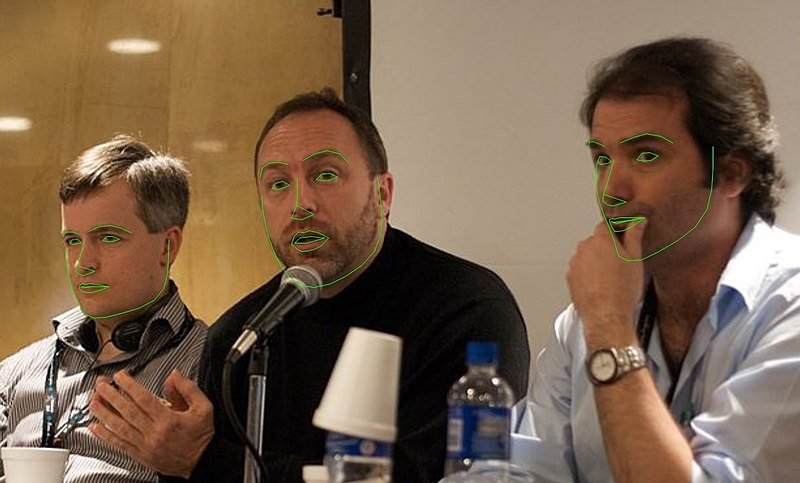
\includegraphics[width=0.7\textwidth]{dlib-face_landmark_detection.jpg}    
    \caption{Detecção de Marcadores Faciais pela biblioteca Dlib. Imagem publicada sob licença Creative Commons\cite{mtheilerDeteccaoMarcadoresFaciais2019}. }
    \label{fig:dlib-landmarking}
\end{figure}

Além disso, a mesma implementa um detector de marcadores faciais baseado em uma floresta de árvores de regressão, capaz de identificar (ou estimar, caso não estejam visíveis) as posições de um conjunto de pontos em um rosto, como mostra a figura \ref{fig:dlib-landmarking}.
A biblioteca fornece também um modelo pré-treinado para este detector para identificação de 68 destes marcadores, sob licença que permite uso acadêmico.
Esta funcionalidade foi chave para a escolha da biblioteca para a implementação do trabalho, visto que permitiu o treinamento do classificador utilizando um conjunto menor de dados, sem preocupações quanto a vieses relacionados às características físicas do locutor.

A biblioteca Dlib foi utilizada em sua versão 19.19.0, compilada a partir do código fonte com suporte para GPU e otimizações referentes à arquitetura da CPU.

\subsection{Tensorflow}
\label{subsec:tf}

Tensorflow\cite{tensorflow2015-whitepaper} é um framework de código aberto para aplicações de aprendizado de máquina.
A biblioteca, construída pela empresa Google, apresenta implementações robustas de diversos algoritmos da área, além de uma API que permite a declaração de uma rede neural em função de suas camadas.
A biblioteca suporta, ainda, o uso de uma ou mais GPUs para treinamento da rede neural, através da biblioteca cuDNN. No trabalho, essa foi utilizada para assistir na modelagem da rede neural, assim como seu treinamento e posterior execução como parte do sistema completo.

A escolha desta biblioteca se deu devido à sua implementação de algoritmos chave para o desenvolvimento do trabalho, tais como a rede neural convolucional tridimensional, discutida na seção \ref{sec:ann}.
Além disso, suas interfaces nas linguagens de programação C++ e Python, assim como a facilidade de utilização de interface em Python para prototipagem rápida de redes neurais convolucionais com topologias diferentes foram decisivas para sua escolha para a realização do trabalho.

Nesse trabalho, utilizamos a versão do Tensorflow 2.1.0, compilada a partir do código fonte com suporte para GPU e otimizações do referentes à arquitetura da CPU.

\subsection{Ambiente de Desenvolvimento}
\label{subsec:environ}

No desenvolvimento deste trabalho foi utilizada em caráter primário a linguagem de programação Python.
Originalmente, o trabalho seria desenvolvido em C++ devido ao mais alto desempenho desta linguagem; no entanto, a utilização de diversas bibliotecas com interface em Python assim como o mais rápido desenvolvimento e prototipagem nesta linguagem levou à decisão final de utiliza-la para a implementação do projeto.

A IDE utilizada no desenvolvimento foi o Visual Studio Code, ferramenta de código aberto criada pela Microsoft, e o Jupyter Notebook\cite{kluyverJupyterNotebooksPublishing2016}, por sua capacidade de subdividir e visualizar o estado do programa em execução.
%O treinamento da rede neural foi realizado em máquina com sistema operacional Windows 10, equipada com uma CPU Intel Core i7 de quarta geração, 12 GB de memória RAM e uma GPU Nvidia GTX 980 com 4 GB de memória dedicada.
O treinamento da rede neural foi realizado em máquina com sistema operacional Ubuntu Linux 16.04, equipada com uma CPU Intel Core i7 de primeira geração, 12 GB de memória RAM, e uma GPU Nvidia GTX 1080 Ti com 12 GB de memória dedicada.

\subsection{Outras Ferramentas}
\label{subsec:otools}

Nesta seção apresentamos as demais bibliotecas utilizadas no desenvolvimento do projeto. Em cada subseção descrevemos brevemente a biblioteca, definindo seu papel no projeto.

As bibliotecas se encontram ordenadas por sua função na pipeline do classificador, discutida de forma mais aprofundada na seção \ref{sec:train}.

\subsubsection{OpenCV}

OpenCV\cite{opencv_library} é uma biblioteca de código aberto para aplicações de Visão Computacional.
Ela foi utilizada para realizar a leitura quadro a quadro dos arquivos de vídeo a serem processados pelo sistema, e para codificar em vídeo a saída do classificador.
Neste trabalho foi utilizada a biblioteca opencv-python em sua versão 4.2.0.32.

\subsubsection{Matplotlib}

A Matplotlib\cite{hunterMatplotlib2DGraphics2007} é uma biblioteca para produção de gráficos e imagens em Python.
Ela foi utilizada para produzir as imagens intermediárias, através do desenho de polígonos a partir dos vértices produzidos pelo processo de detecção de marcadores facial.
Neste trabalho utilizamos a Matplotlib na versão 3.1.3 da biblioteca.

\subsubsection{Pandas}

Pandas\cite{mckinney-proc-scipy-2010} é uma biblioteca de processamento de dados em Python.
Ela foi utilizada no pré-processamento dos dados com a finalidade de manipular os arquivos csv contendo a diarização manual dos vídeos do dataset de depoimentos.
A biblioteca foi utilizada em sua versão 1.0.0.

\subsubsection{Scikit Learn e dscore}

As bibliotecas Scikit-Learn\cite{pedregosaScikitlearnMachineLearning2011}, biblioteca de aprendizado de máquina tradicional em python, e dscore\cite{ryantNryantDscore2020}, biblioteca para cálculo de métricas de diarização, foram utilizadas para o cálculo de diversas métricas relacionadas ao desempenho do sistema.
Essas foram utilizadas em suas versões 0.22.2.post1 e 1.1.0, respectivamente.

\section{Preparação dos Dados}
\label{sec:preproc}

Originalmente, foi fornecido pela Defensoria Pública do Estado do Rio de Janeiro um dataset contendo 29 vídeos, totalizando cerca de 5 horas de vídeo, referente a depoimentos prestados por diferentes participantes.
Os vídeos fornecidos apresentam resolução de $320\times240$ pixels, a uma taxa de 30 quadros por segundo.
O conjunto de dados não apresentava nenhuma anotação referente à fala dos depoentes.

Primeiramente, segmentamos os vídeos em fragmentos de 15 quadros, ou meio segundo.
A motivação para a segmentação do vídeo de entrada em trechos deste comprimento foi a estipulação de que o tempo necessário para a fala da primeira sílaba em uma frase, por uma pessoa normal, no português do Brasil, é de 252 milissegundos\cite{barbosaSyllabletimingBrazilianPortuguese2000}.
Sendo assim, ao dobrar este tempo, adquirimos a capacidade de detectar por completo o movimento do locutor quando referente a frases curtas, tais como interjeições.

Estes trechos foram validados para determinar se a face do depoente poderia ser reconhecida, com finalidade de descartar fragmentos nos quais este não olhava em direção à câmera, ou nas quais o detector HOG não poderia identifica-los.
Cada trecho foi então manualmente classificado quanto à ocorrência de fala pelo depoente, produzindo uma tabela que associava o identificador de cada arquivo à classe correspondente ao mesmo.

Feita essa diarização manual, os vídeos foram separados em conjuntos de treinamento e teste, tal que fragmentos provenientes de um mesmo vídeo nunca seriam utilizados em ambas as fases do processo.
Fizemos essa separação pois, como os fragmentos possuem relação temporal tanto entre si quanto com outros vídeos do mesmo depoente, seria possível que o treinamento da rede neural utilizando segmentos semelhantes aos fragmentos de teste pudesse inflar artificialmente o desempenho da mesma.

Para a execução de todas essas tarefas foram desenvolvidos scripts em Python e Bash, capazes de segmentar os vídeos do dataset e de validar, mover, e organizar os fragmentos extraídos destes.

\section{Treinamento}
\label{sec:train}

Para o treinamento do modelo foi desenvolvido um sistema composto por dois componentes principais.

\begin{figure}[ht]
    \centering
    \fontsize{10pt}{10pt}\selectfont
    \includesvg[width=0.95\textwidth]{figures/architecture.svg}
    %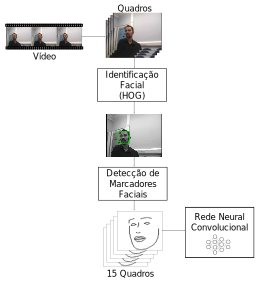
\includegraphics[width=0.85\textwidth]{figures/architecture.png}
    \caption{A sequência de carregamento dos dados e treinamento do modelo.}
    \label{fig:arch_train}
\end{figure}

Primeiramente, foi construído um gerador de dados com a finalidade de alimentar os dados da entrada ao modelo dinamicamente. As características e funcionalidades se encontram descritas na seção \ref{sec:data-gen}.
Depois, foi definida a topologia do modelo de rede neural, discutida na seção \ref{sec:topology}, e os critérios e parâmetros relevantes ao fluxo de treinamento, discutidos na seção \ref{sec:train-flow}.

\subsection{Carregador de Dados}
\label{sec:data-gen}
A função primária do carregador de dados é ler dinamicamente os vídeos a serem alimentados ao modelo em cada etapa de seu treinamento.
Um módulo capaz de realizar tal carregamento dinâmico foi necessário devido ao grande volume de dados sendo processados, por virtude de se tratarem de dados de vídeo.
Para isto, ele é inicializado com uma lista dos arquivos a serem carregados, assim como uma série de parâmetros que definem aspectos de sua operação, tais como o tamanho da batelada ou o pré-processamento a ser aplicado aos quadros.

Cada vídeo fornecido ao carregador é, ainda, invertido horizontalmente.
Isso é feito para garantir que o modelo fosse treinado para funcionar independentemente do ângulo do rosto do sujeito, desde que reconhecível pelo HOG, visto que na grande maioria dos vídeos do dataset original o falante se encontrava olhando para o lado esquerdo da câmera ou diretamente para esta.

Para acelerar o processo de identificação facial e detecção de marcadores faciais, o carregador é capaz de processar múltiplos fragmentos em paralelo na CPU, além de manter um cache dos fragmentos processados em iterações anteriores do treinamento.
Esse paralelismo possibilitou a redução do tempo de execução da primeira iteração do treinamento e teste de cerca de 9 horas para aproximadamente uma hora e trinta minutos, uma redução de 83\% no tempo de execução com 6 threads, enquanto a implementação do cache reduziu o tempo necessário para etapas subsequentes do processo de para cerca de 3 minutos.

\subsection{Pré-Processamento}
\label{sec:pre-processing}

O carregador de dados possui 3 modos distintos de operação, demonstrados na figura \ref{fig:generator_out}, que correspondem aos filtros de pré-processamento que podem ser aplicados aos quadros carregados para compor a entrada do modelo de predição. Estes são:

\begin{enumerate}[label={(\arabic*)}]
    \item RGB: Nesse modo, o quadro é codificado em padrão RGB, ou seja, com cores representadas por suas componentes vermelha, verde, e azul, nessa ordem.
    \item Grayscale: Nesse modo, o quadro RGB é convertido para escala de cinza, segundo a função $Y = 0.299 R + 0.587 G + 0.114 B$.
    \item Landmarks: Nesse modo, é gerada uma imagem em preto e branco, rasterizada a partir dos pontos identificados pela detecção de marcadores faciais em cada quadro carregado. Este foi o modo utilizado na implementação final do trabalho.
\end{enumerate}

\begin{figure}[ht]
    \centering
    \begin{enumerate}[label={(\arabic*)}]
        \item \parbox{\linewidth}{\centering
            \includesvg[width=0.9\textwidth]{loader_rgb.svg}
        }
        \item \parbox{\linewidth}{\centering
            \includesvg[width=0.9\textwidth]{loader_gray.svg}
        }
        \item \parbox{\linewidth}{\centering
            \includesvg[width=0.9\textwidth]{loader_lm.svg}
        }
    \end{enumerate}
    \caption{A saída do carregador de dados em cada um de seus três modos de operação.}
    \label{fig:generator_out}
\end{figure}

\begin{algorithm}[H]
    \SetAlgoLined
    \caption{Pré-processamento de um fragmento de vídeo (landmarks).}
    \label{alg:pre-processing}
    \KwResult{Sequência de 15 quadros pré-processados}
    \While{Quadros Carregados < 15}{
        Carrega quadro do fragmento\;
        Detecta faces no quadro carregado usando o detector facial (HOG)\;
        Calcula os 68 marcadores faciais utilizando o algoritmo de alinhamento facial\;
        Rasteriza os marcadores obtidos sobre um canvas branco\;
        Recorta o canvas segundo a região identificada pelo HOG\;
        Alinha horizontalmente a face detectada e amplia o desenho\;
    }
\end{algorithm}

Em nossa implementação final, utilizamos o modo de \textit{landmarks}. Esse modo implementa o algoritmo \ref{alg:pre-processing}.

\subsection{Topologia do Modelo}
\label{sec:topology}

Para o modelo de predição, definimos uma topologia baseada na arquitetura VGG\footnote{VGG é um estilo de arquitetura de rede neural convolucional para reconhecimento de objetos em fotos, desenvolvida pelo Grupo de Geometria Visual (do inglês \textit{Visual Geometry Group}) da universidade de Oxford \cite{simonyanVeryDeepConvolutional2015}.}, definido na figura \ref{fig:topology_typeA}, que consiste em um número de pares de camadas de convolução e \textit{max pooling}, seguidas de camadas densamente conectadas.
A arquitetura foi adaptada para lidar com dados de caráter tri-dimensional.
Nesta seção iremos discutir as decisões tomadas neste processo de adaptação da arquitetura, e os fatores que levaram a estas decisões.

\begin{figure}[ht]
    \centering
    \resizebox{!}{0.7\textheight}{
        \newcommand{\GenericLayer}[5]{
    \begin{minipage}{0.3\textwidth}
        \centering
        \baselineskip=1.25\baselineskip
            {\footnotesize{#2} \hfill \footnotesize{#3} \hfill \footnotesize{#4}}%
            \linebreak
            {\textbf{#1}}%
            \linebreak
            {\small{#5}}
    \end{minipage}%
}
\newcommand{\BasicLayer}[2]{
    \begin{minipage}{0.3\textwidth}
        \centering
        \baselineskip=1.25\baselineskip
            {\textbf{#1}}%
            \linebreak
            {\small{#2}}
    \end{minipage}%
}
\newcommand{\ConvLayer}[4]{
    \GenericLayer{#1}{K: (#2)}{}{\textbf{F: #3}}{#4}%
}
\newcommand{\PoolLayer}[3]{
    \GenericLayer{#1}{S: #2}{}{}{#3}%
}
\newcommand{\DenseLayer}[2]{
    \BasicLayer{#1}{S: #2}%
}
\newcommand{\InputLayer}[2]{
    \BasicLayer{#1}{#2}%
}

\begin{tikzpicture}[]
    \node[state, rectangle, align=center, fill=blue!20!white] (input) [] {
        \InputLayer{Entrada}{$15\times150\times150$}%
    };
    \node[state, rectangle, align=center] (conv3d_1) [below=of input] {
        \ConvLayer{Convolução 3D}{$4\times3\times3$}{16}{$12\times148\times148$}%
    };
    \node[state, rectangle, align=center] (maxpool_1) [below=of conv3d_1] {
        \PoolLayer{Max Pooling 3D}{$(2\times2\times2)$}{$6\times74\times74$}%
    };
    \node[state, rectangle, align=center] (conv3d_2) [below=of maxpool_1] {
        \ConvLayer{Convolução 3D}{$3\times3\times3$}{32}{$4\times72\times72$}%
    };
    \node[state, rectangle, align=center] (maxpool_2) [below=of conv3d_2] {
        \PoolLayer{Max Pooling 3D}{$(2\times2\times2)$}{$2\times36\times36$}%
    };
    \node[state, rectangle, align=center] (conv3d_3) [below=of maxpool_2] {
        \ConvLayer{Convolução 3D}{$1\times3\times3$}{64}{$2\times34\times34$}%
    };
    \node[state, rectangle, align=center] (maxpool_3) [below=of conv3d_3] {
        \PoolLayer{Max Pooling 3D}{$(2\times2\times2)$}{$1\times17\times17$}%
    };
    \node[state, rectangle, align=center] (dense_1) [below=of maxpool_3] {
        \DenseLayer{Densa}{$256$}%
    };
    \node[state, rectangle, align=center] (dense_2) [below=of dense_1] {
        \DenseLayer{Densa}{$128$}%
    };
    \node[state, rectangle, align=center, fill=green!20!white] (sofmax) [below=of dense_2] {
        \DenseLayer{Softmax}{$2$}%
    };
    
    \draw[-{Latex[length=2mm]}] (input) -- (conv3d_1);
    \draw[-{Latex[length=2mm]}] (conv3d_1) -- (maxpool_1);
    \draw[-{Latex[length=2mm]}] (maxpool_1) -- (conv3d_2);
    \draw[-{Latex[length=2mm]}] (conv3d_2) -- (maxpool_2);
    \draw[-{Latex[length=2mm]}] (maxpool_2) -- (conv3d_3);
    \draw[-{Latex[length=2mm]}] (conv3d_3) -- (maxpool_3);
    \draw[-{Latex[length=2mm]}] (maxpool_3) -- (dense_1);
    \draw[-{Latex[length=2mm]}] (dense_1) -- (dense_2);
    \draw[-{Latex[length=2mm]}] (dense_2) -- (sofmax);
    
    \node[state, rectangle, yshift=-1.1cm, fill=red!20!white] (dropout_1) [right=of input] {
        \DenseLayer{Dropout Espacial}{$40\%$}%
    };
    \node[state, rectangle, yshift=-1.5cm, fill=red!20!white] (dropout_2) [right=of maxpool_2] {
        \DenseLayer{Dropout Espacial}{$35\%$}%
    };
    \node[state, rectangle, yshift=-1.5cm, fill=red!20!white] (dropout_3) [right=of maxpool_3] {
        \DenseLayer{Dropout}{$50\%$}%
    };
    \node[state, rectangle, yshift=-1.1cm, fill=red!20!white] (dropout_4) [right=of dense_1] {
        \DenseLayer{Dropout}{$25\%$}%
    };
    
    \draw[-{Latex[length=2mm]}] (dropout_1) |- (conv3d_1);
    \draw[-{Latex[length=2mm]}] (dropout_1) |- (conv3d_2);
    \draw[-{Latex[length=2mm]}] (dropout_2) |- (conv3d_3);
    
    \draw[-{Latex[length=2mm]}] (dropout_3) |- (dense_1);
    \draw[-{Latex[length=2mm]}] (dropout_4) |- (dense_2);
    
    \node[draw=none, fill=none, minimum size=0.3\textwidth] [left=of input] (placeholder) {};
\end{tikzpicture}
        }
    \caption{Topologia do Modelo}
    \label{fig:topology_typeA}
\end{figure}

Primeiramente, na primeira camada convolucional da rede, que frequentemente tem a função de detectar bordas na imagem de entrada, adicionamos uma componente temporal ao \kernel\ com dimensão 4.
Essa dimensão par não é usual para uma rede neural convolucional, que tradicionalmente busca identificar padrões nas vizinhanças de cada elemento, devido ao fato de que não atua sobre um elemento da imagem original alterando-o em relação a seus vizinhos.
Ao invés disso, a dimensão par produz um novo elemento, localizado espacialmente em seu centro, e cujo valor é obtido a partir da média ponderada pelos pesos do \kernel\ de células da entrada.
Em nosso modelo isso corresponde a construir um conjunto de filtros capazes de identificar variações temporais relevantes em cada sequência de 4 quadros da entrada.

Na segunda camada de convolução, adicionamos uma componente temporal com dimensão 3, igual às demais.
Isto consiste em avaliar o valor de cada ponto da matriz de entrada em função dos valores de seus vizinhos, o que possibilita a identificação das áreas da matriz relevantes ao problema.
A baixa dimensão utilizada em relação ao tamanho da entrada faz com que as características observadas sejam características locais, tais como bordas e cantos nas quais ocorram as variações desejadas já previamente identificadas.

Na última camada de convolução, mantivemos caráter bi-dimensional do \kernel\ através da dimensão temporal igual a 1, apesar de constituir uma convolução tri-dimensional.
Isso corresponde a operar individualmente sobre os quadros da entrada, agora compostos pela combinação temporal dos quadros originais, buscando características destes que sejam relevantes para a classificação, a ser realizada em seguida pelas camadas densas.

Finalmente, o número de neurônios das camadas totalmente conectadas foi reduzido a partir dos valores originais propostos na VGG16.
Essa redução foi realizada de forma iterativa, buscando manter a acurácia do modelo constante e reduzir o \textit{overfitting} através da eliminação de parâmetros redundantes.

\subsection{Treinamento do Modelo}
\label{sec:train-flow}

Em cada época, o sistema de treinamento do modelo chama o carregador de dados de treinamento, que lhe retorna um número fixo de amostras (batelada) compostas por segmentos de 15 quadros consecutivos.
O modelo então faz suas predições quanto a estas, e tem seus pesos ajustados através do algoritmo de retro-propagação de forma a minimizar uma função de custo.

\begin{equation} \label{eq:categorical_crossentropy}
    L(y,\hat{y})=-\sum\limits_{j=0}^M\sum\limits_{i=0}^N(y_{ij}*log(\hat{y}_{ij}))
\end{equation}

Como se trata de um problema de classificação, escolhemos como função custo do treinamento a função de entropia categórica cruzada, definida na equação \ref{eq:categorical_crossentropy}. Nessa equação, $\hat{y}$ é o vetor das probabilidades das categorias, e $y$ é a categoria real, codificada \textit{one-hot}\footnote{Codificação \textit{one-hot} é uma forma de representar a classe dentre um conjunto de classes à qual um item pertence, na forma de uma sequência binária na qual um único bit, correspondente a esta, esteja no nível lógico 1.}.

Visto que trata-se um problema de classificação binária, seria possível também utilizar a função de entropia cruzada binária; Porém, considerando a possibilidade de expansão futura do modelo para detecção de outras ações conversacionais, tais como gestos com a cabeça, decidimos utilizar uma função custo escalável para adição de novas classes.

Como forma de reduzir o \textit{overfitting} da rede neural aos dados do treinamento, aplicamos \textit{Dropout}\footnote{\textit{Dropout} é uma técnica que consiste na remoção aleatória de neurônios temporariamente de uma camada da rede neural durante o treinamento. \textit{Dropout Espacial} é uma variação desta técnica, que consiste em remover neurônios agrupados por região espacial.} às camadas totalmente conectadas desta, e \textit{Dropout Espacial} à saída de suas camadas convolucionais.
A figura \ref{fig:training_metrics} mostra o resultado da utilização dessas técnicas no treinamento do modelo.

\begin{figure}[ht]
    \centering
    \resizebox{0.95\textwidth}{!}{
        \begin{tabular}{cc}
    Custo Treinamento & Acurácia Treinamento \\
    \begin{tikzpicture}
        \begin{axis}[xmin=0, ymin=0, xmax=50, ymax=2, every axis plot/.append style={very thick}, minor tick num=5, grid=both, grid style={line width=.1pt, draw=gray!10}, no markers]
            \addplot table [x=Step, y=Value, col sep=comma] {figures/run-2020-05-21-2357_train-tag-epoch_loss.csv};
            \addplot table [x=Step, y=Value, col sep=comma] {figures/run-2020-05-29-1814_train-tag-epoch_loss.csv};
        \end{axis}
    \end{tikzpicture} 
    &
    \begin{tikzpicture}
        \begin{axis}[xmin=0, ymin=0, xmax=50, ymax=1, every axis plot/.append style={very thick}, minor tick num=5, grid=both, grid style={line width=.1pt, draw=gray!10}, no markers]
            \addplot table [x=Step, y=Value, col sep=comma] {figures/run-2020-05-21-2357_train-tag-epoch_basics_accuracy.csv};
            \addplot table [x=Step, y=Value, col sep=comma] {figures/run-2020-05-29-1814_train-tag-epoch_basics_accuracy.csv};
        \end{axis}
    \end{tikzpicture} 
    \\
    \begin{tikzpicture}
        \begin{axis}[xmin=0, ymin=0, xmax=50, ymax=2, every axis plot/.append style={very thick}, minor tick num=5, grid=both, grid style={line width=.1pt, draw=gray!10}, no markers]
            \addplot table [x=Step, y=Value, col sep=comma] {figures/run-2020-05-21-2357_validation-tag-epoch_loss.csv};
            \addplot table [x=Step, y=Value, col sep=comma] {figures/run-2020-05-29-1814_validation-tag-epoch_loss.csv};
        \end{axis}
    \end{tikzpicture} 
    &
    \begin{tikzpicture}
        \begin{axis}[xmin=0, ymin=0, xmax=50, ymax=1, every axis plot/.append style={very thick}, minor tick num=5, grid=both, grid style={line width=.1pt, draw=gray!10}, legend style={at={(0.98,0.02)},anchor=south east}, no markers]
            \addplot table [x=Step, y=Value, col sep=comma] {figures/run-2020-05-21-2357_validation-tag-epoch_basics_accuracy.csv};
            \addlegendentry{Com \textit{Dropout}}
            
            \addplot table [x=Step, y=Value, col sep=comma] {figures/run-2020-05-29-1814_validation-tag-epoch_basics_accuracy.csv};
            \addlegendentry{Sem \textit{Dropout}}
        \end{axis}
    \end{tikzpicture} 
    \\
     Custo Validação & Acurácia Validação \\
\end{tabular}
    }
    \caption{Evolução das métricas de desempenho ao longo dos processos de treinamento e validação do modelo, com e sem \textit{dropout}, representado pelas linhas azul e vermelha respectivamente. Note que, sem \textit{dropout}, a acurácia no conjunto de treinamento tende a 1 e sua função custo tende a 0, enquanto a função custo no conjunto de validação não converge. }
    \label{fig:training_metrics}
\end{figure}

Além disso, aplicamos regularização L2 sobre o \kernel\ e \textit{bias} de todas as camadas da rede.
Essa regularização consiste em acrescentar uma penalidade sobre o ajuste do valor de ativação de cada neurônio $x_i$, definida na equação \ref{eq:l2_regularization}, ao valor da função custo definida anteriormente.

\begin{equation}\label{eq:l2_regularization}
    p_{l_2} = l_2 \sum\limits_{i=0}^n(x_i)^2
\end{equation}

Uma vez esgotadas as amostras de treinamento, o modelo chama, então, o carregador de dados de validação, realizando predições sem retro-propagação sobre as entradas retornadas, e calculando o valor da função custo para os resultados.
Esta etapa é fundamental para garantirmos que o modelo treinado seja aplicável a dados do mundo real, e não exclusivamente aos dados do conjunto de treinamento.

Por fim, ao se esgotarem também essas amostras, dá-se o final de uma época do treinamento, e os carregadores tem suas listas de arquivos embaralhadas de forma a garantir aleatoriedade na ordem da próxima época.
Ainda para prevenção de \textit{overfitting} na rede neural foi definido como critério de parada do treinamento a condição de que não haja redução da função custo durante cinquenta épocas do treinamento.

\section{Aplicação}
\label{sec:application}

A aplicação de diarização resultante deste trabalho é capaz de, quando executada sobre um arquivo de vídeo, diarizar o mesmo produzindo um arquivo em formato RTTM\footnote{O formato RTTM, do inglês \textit{Rich Transcription Time Marked}, é um formato de arquivo texto definido pela NIST em 2009 para representação de transcrições. Sua especificação formal pode ser encontrada em \cite{nist2009RT09Rich2009}, publicado pela organização.} identificando os períodos correspondentes à fala do orador. 
Essa aplicação implementa o algoritmo \ref{alg:application}, que define uma janela deslizante que percorre o vídeo de entrada, avançando a cada iteração um número fixo de quadros determinado pelo parâmetro \textit{step}.
A figura \ref{fig:alg_demo} demonstra a execuçã das duas primeiras iterações do algoritmo para a diarização de uma mídia completa.

\begin{algorithm}[ht]
    \SetAlgoLined
    \caption{Algoritmo de diarização de mídia.}
    \label{alg:application}
    \KwResult{Diarização completa da mídia de entrada.}
    \While{Mídia de entrada possui quadros}{
        \While{Quadros Carregados < 15}{
            Carrega quadro da mídia de entrada\;
            Aplica pré-processamento sobre o quadro carregado\;
            Adiciona quadro carregado à janela\;
        }
        Realiza predição sobre os quadros da janela utilizando o modelo classificador\;
        Armazena resultado em listas correspondentes aos quadros\;
        Consolida os $step$ quadros mais antigos\;
        Descarta os $step$ quadros mais antigos\;
    }
\end{algorithm}

\begin{figure}[ht]
    \centering
    %\input{figures/alg_demo.tikz}
    \begin{subfigure}[b]{\textwidth}
        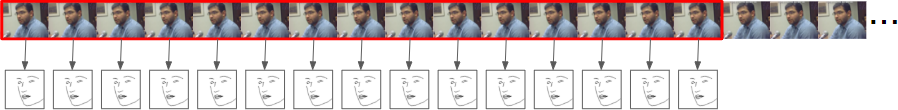
\includegraphics[width=\textwidth]{figures/alg_demo_2.png}
        \caption{Os 15 primeiros quadros são carregados e pré-processados, produzindo bitmaps traçados a partir dos marcadores faciais detectados.}
    \end{subfigure}
    \newline
    \newline
    \begin{subfigure}[b]{\textwidth}
        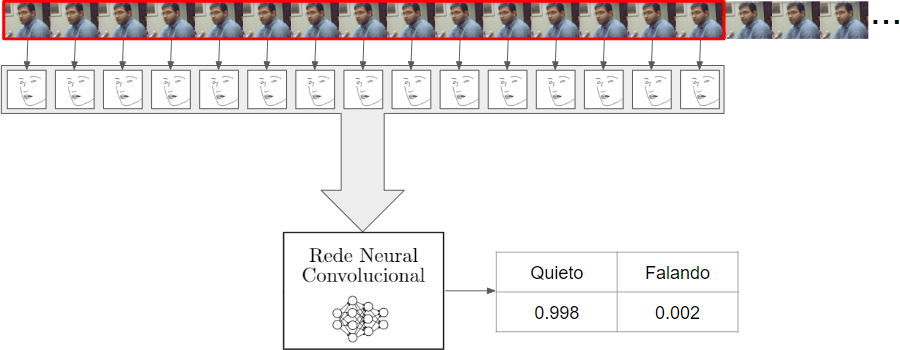
\includegraphics[width=\textwidth]{figures/alg_demo_4.png}
        \caption{A janela é classificada pela rede neural, que retorna as probabilidades de cada classe para essa.}
    \end{subfigure}
    \newline
    \newline
    \begin{subfigure}[b]{\textwidth}
        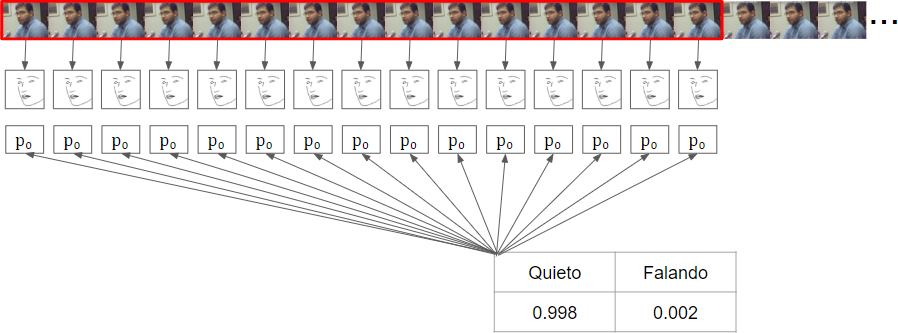
\includegraphics[width=\textwidth]{figures/alg_demo_5.png}
        \caption{As probabilidades retornadas pelo classificador são associadas a cada um dos quadros.}
    \end{subfigure}
    \newline
    \newline
    \begin{subfigure}[b]{\textwidth}
        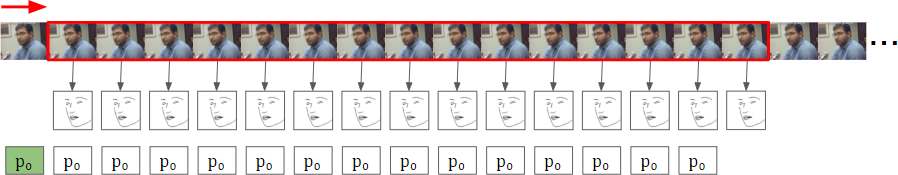
\includegraphics[width=\textwidth]{figures/alg_demo_7.png}
        \caption{A janela desliza um quadro para a direita, e o próximo quadro é pré-processado. Como o quadro que saiu da janela possui apenas uma classificação, a classe com maior probabilidade é utilizada.}
    \end{subfigure}
    \caption{Demonstração do funcionamento do algoritmo para as duas primeiras iterações do processo de diarização de uma mídia completa com $step = 1$.}
\end{figure}

\begin{figure}[ht]\ContinuedFloat
    \centering
    \begin{subfigure}[b]{\textwidth}
        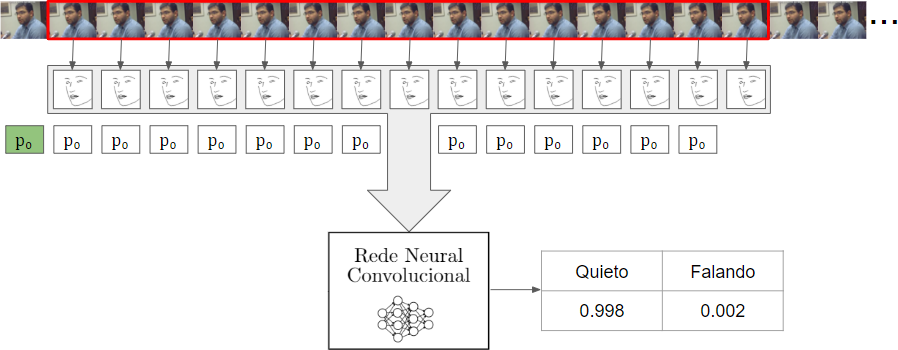
\includegraphics[width=\textwidth]{figures/alg_demo_9.png}
        \caption{A nova janela é classificada pela rede neural, produzindo um novo conjunto de probabilidades.}
    \end{subfigure}
    \newline
    \newline
    \newline
    \begin{subfigure}[b]{\textwidth}
        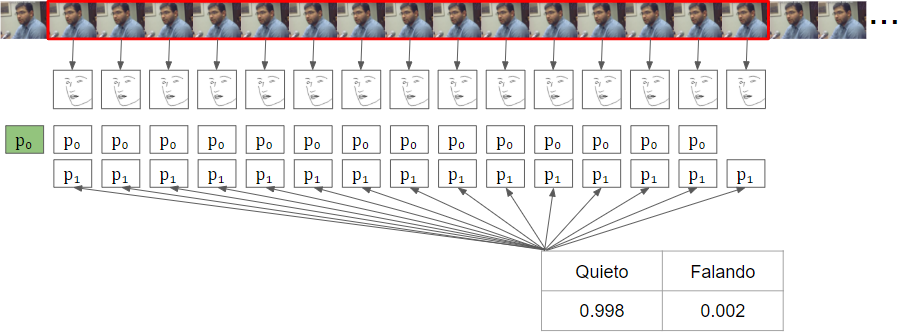
\includegraphics[width=\textwidth]{figures/alg_demo_10.png}
        \caption{As probabilidades retornadas pelo classificador são associadas a cada um dos quadros.}
    \end{subfigure}
    \begin{subfigure}[b]{\textwidth}
        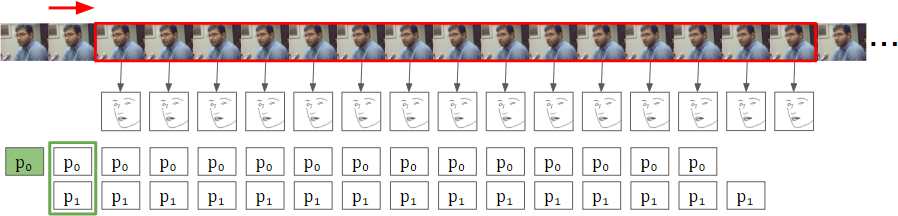
\includegraphics[width=\textwidth]{figures/alg_demo_12.png}
        \caption{A janela desliza outro quadro para a direita, e o próximo quadro é pré-processado. Como o quadro que saiu da janela possui mais de uma classificação, suas probabilidades são consolidadas segundo o algoritmo selecionado.}
    \end{subfigure}
    \caption{Demonstração do funcionamento do algoritmo para as duas primeiras iterações do processo de diarização de uma mídia completa com $step = 1$.}
    \label{fig:alg_demo}
\end{figure}

O algoritmo utilizado para pré-processamento dos quadros já foi discutido na seção \ref{sec:pre-processing}, e as características do modelo de classificação foram discutidas na seção \ref{sec:topology}.
Sendo assim, discutiremos nesta seção, primariamente, as considerações feitas durante o processo de desenvolvimento da aplicação quanto ao algoritmo utilizado para consolidação das predições realizadas para os quadros individuais, e o fluxo de erro adotado quando não é possível obter uma classificação para um determinado quadro.

\subsection{Consolidação das Classificações}
\label{sec:class-commit}

Com a finalidade de obter maior precisão temporal do que seria possível apenas com a classificação de sequências de 15 quadros, a diarização é feita com tamanho de passo $step \leq 15$ tal que cada quadro passe pelo classificador um número $n = \floor{15 / step}$ de vezes, em diferentes posições no fragmento.
Dessa forma, torna-se necessário consolidar as diversas predições realizadas sobre cada quadro ao adiciona-los à transcrição final.

Para esse processo, implementamos 5 algoritmos distintos. 
Estes consistem em funções que, quando aplicadas a um conjunto de predições de tamanho variável, retornam um único conjunto de confianças correspondentes a cada classe alvo.
Com esse propósito, implementamos as funções \textit{valor central}, \textit{média}, \textit{frequência de predição}, \textit{média gaussiana}, e \textit{frequência gaussiana}.
A classe de maior confiança retornada por estes algoritmos é considerada a classe real do quadro, e é adicionada à diarização.

\subsubsection{Valor Central}

O algoritmo de valor central é o algoritmo de consolidação mais simples entre os algoritmos implementados.
Este consiste em selecionar as confianças de cada classe referentes à predição realizada com o quadro no centro do fragmento.

\subsubsection{Média}

Este algoritmo consiste em calcular a média aritmética das confianças retornadas pela camada \textit{softmax} do modelo preditor para cada classe.
Essa média é utilizada como nova confiança do quadro.

\subsubsection{Frequência}

O algoritmo de frequência é bastante semelhante ao algoritmo de média, no entanto ao invés de fazer uso das confianças retornadas pelo modelo este considera as predições deste absolutas e seleciona a predição mais frequente para cada quadro individual.

\subsubsection{Média e Frequência Gaussiana}

Estes algoritmos consistem em implementações dos algoritmos de média e frequência já analisados anteriormente nas quais os valores das predições individuais são ponderados a partir de pesos obtidos a partir de valores de uma distribuição normal (equação \ref{eq:normal-dist}) em $\floor{15 / step}$ pontos distribuídos linearmente em $[-2, 2]$.

\begin{equation}\label{eq:normal-dist}
    \varphi = \frac{1}{\sqrt{2\pi}} e ^ {\frac{-x^2}{2}}
\end{equation}

A intuição por trás da inclusão destes algoritmos foi de que predições realizadas com o quadro em questão próximo ao centro do fragmento seriam mais representativas da real classe desse do que predições realizadas com o mesmo nas extremidades do fragmento.
O uso de uma distribuição normal, então, enfatizaria as confianças ou frequências dessas classificações.

\subsection{Fluxo de Erro e Dados Ausentes}
\label{sec:missing-data}

Caracterizamos como dado ausente todo quadros no qual o algoritmo de detecção facial não é capaz de detectar um rosto na imagem.
Isso pode ocorrer em diversas situações, desde um movimento por parte do orador que esconda sua face até sua real ausência na gravação.
Note que neste momento não consideramos detecções incorretas como um dado ausente.

Uma vez que o diarizador encontra um dado ausente, torna-se impossível completar uma sequência de 15 quadros para a realização de novas classificações.
É necessário, então, consolidar as predições quanto a todos os quadros já feitas anteriormente.
Isso é feito utilizando os mesmos algoritmos já discutidos na seção \ref{sec:class-commit}.

O quadro que iniciou o erro é, então adicionado à diarização com classe desconhecida.
Quadros subsequentes que também não possuam faces identificáveis incrementam a duração deste trecho de diarização desconhecida.
Uma vez carregados consecutivamente 15 novos quadros válidos, essa é encerrada e o diarizador retorna ao fluxo normal.

Adicionalmente, é também considerado com erro qualquer quadro que, ao ter suas classificações consolidadas, apresente confianças iguais para duas ou mais classes.
\chapter{Resultados}
\label{chap:results}

Neste capítulo discutiremos os resultados obtidos nos testes realizados com o sistema diarizador.
Primeiramente, na seção \ref{sec:results-model}, discutiremos os resultados referentes ao modelo classificador treinado como componente preditora do sistema.
Depois, na seção \ref{sec:results-app}, apresentaremos os resultados referentes à aplicação diarizadora como um todo.

\section{Modelo Classificador}
\label{sec:results-model}

Nesta seção avaliaremos o desempenho do modelo treinado em relação à sua capacidade de classificar corretamente segmentos de vídeo de 15 quadros.
Para essa finalidade, utilizamos os segmentos de 2 vídeos distintos do dataset que não foram utilizados anteriormente durante o treinamento do modelo, totalizando 990 segmentos válidos com duração de meio segundo e classificados manualmente.
Além disso, utilizamos também versões destes espelhadas horizontalmente, totalizando 1980 amostras totais para teste do modelo.

Na seção \ref{sec:results-model-gen} apresentamos as métricas gerais de desempenho do modelo, e na seção \ref{sec:results-model-confusion} apresentamos as métricas de confusão, referentes ao desempenho deste em relação a cada uma das classes alvo.
Todas as métricas serão apresentadas para 3 conjuntos de pesos distintos obtidos durante o processo treinamento do modelo. Estes são:
\begin{itemize}
    \item Os pesos que minimizam o valor da custo utilizada;
    \item Os pesos que maximizam o valor da acurácia do modelo;
    \item Os pesos obtidos ao final de todas as épocas do treinamento.
\end{itemize}

\subsection{Métricas Gerais}
\label{sec:results-model-gen}

As métricas gerais calculadas para o modelo incluem a sua acurácia, que representa a capacidade do modelo de classificar um dado segmento de video corretamente, a entropia categórica (equação \ref{eq:categorical_crossentropy}), que corresponde à certeza do modelo quanto a suas predições, e a área abaixo da curva ROC.
A figura \ref{fig:general-metrics-val} mostra a evolução dessas métricas ao longo do processo de treinamento do modelo, enquanto a tabela \ref{tab:general-metrics-val} destaca os valores destas métricas para os conjuntos de pesos obtidos ao final do treinamento.

\begin{figure}[ht]
    \centering
    \begin{tikzpicture}
        \begin{axis}[xmin=0, ymin=0, xmax=68, ymax=1, width=0.65\textwidth, every axis plot/.append style={very thick}, minor tick num=5, grid=both, grid style={line width=.1pt, draw=gray!10}, legend style={at={(1.18,0.02)},anchor=south east}, no markers, legend cell align={left}]
            \addplot table [x=Step, y=Value, col sep=comma] {figures/run-2020-05-21-2357_validation-tag-epoch_basics_accuracy.csv};
            \addlegendentry{Acurácia}
            \addplot[OliveGreen] table [x=Step, y=Value, col sep=comma] {figures/run-2020-05-21-2357_validation-tag-epoch_basics_auc.csv};
            \addlegendentry{Area Under Curve}
            \addplot[red] table [x=Step, y=Value, col sep=comma] {figures/run-2020-05-21-2357_validation-tag-epoch_basics_cce.csv};
            \addlegendentry{Entropia Categórica}
        \end{axis}
    \end{tikzpicture}
    \caption{Evolução das métricas gerais sobre o conjunto de validação\\ durante o treinamento do modelo. A linha azul representa a evolução da acurácia, enquanto a linha verde corresponde à evolução da área abaixo da curva ROC, e a linha vermelha à da entropia categórica cruzada.}
    \label{fig:general-metrics-val}
\end{figure}

\begin{table}[ht]
    \centering
    \begin{tabular}{|c|c|c|c|c|}
        \rule{1cm}{0pt}&\rule{1.5cm}{0pt}&\rule{1.5cm}{0pt}&\rule{1.5cm}{0pt}&\rule{1cm}{0pt}\\[-\arraystretch\normalbaselineskip]
        \hline
        Pesos & Época & Acurácia & AUC & Entropia Categórica \\
        \hline
        \hline
        Custo Mínimo & 18 & 0.8596 & 0.9314 & 0.3382 \\
        \hline
        Acurácia Máxima & 39 & 0.8656 & 0.9336 & 0.3429 \\
        \hline
        Final & 68 & 0.8561 & 0.9236 & 0.4198 \\
        \hline
    \end{tabular}
    \caption{Métricas referentes aos conjuntos de pesos obtidos ao final\\ do processo de treinamento.}
    \label{tab:general-metrics-val}
\end{table}

\subsection{Métricas de Confusão}
\label{sec:results-model-confusion}

As métricas de confusão demonstram a capacidade do modelo de classificar corretamente os itens pertencentes a cada uma das classes.
Essas incluem a matriz de confusão, que visualiza as classificações feitas pelo diarizador em relação à classe real de cada item, revelando as tendências deste, e os valores de precisão, \textit{recall}, e \textit{$F_1$ Score} calculados a partir desta.

\begin{figure}[ht]
    \centering
    \resizebox{0.9\textwidth}{!}{
        \begin{tabular}{cc}
            \MakeConfusionMatrix{855}{93}{185}{847} & \MakeConfusionMatrix{845}{103}{163}{869} \\
            Menor Custo & Maior Acurácia \\
            & \\
            \multicolumn{2}{c}{\MakeConfusionMatrix{872}{76}{209}{823}} \\
            \multicolumn{2}{c}{Final}
        \end{tabular}
    }
    \caption{Matrizes de Confusão para os conjuntos de pesos obtidos ao final \\ do treinamento do modelo. }
    \label{fig:confusion_matrices}
\end{figure}

A figura \ref{fig:confusion_matrices} mostra as matrizes de confusão dos conjuntos de pesos treinados que obtiveram melhor desempenho sobre o conjunto de treinamento.
Observa-se a acurácia do modelo no percentual de valores que se encontram da diagonal principal desta; Esses valores correspondem às classificações corretas dos elementos de cada classe.
Note, ainda, que os conjuntos de pesos de menor custo e finais do treinamento tendem à esquerda, indicando uma tendência do modelo a classificar negativamente os segmentos observados.

Além disso, para melhor entendimento das propriedades do modelo treinado, calculamos a precisão e o \textit{recall} correspondente a cada classe, assim como o \textit{$F_1$ Score} para os conjuntos de pesos obtidos ao final do processo de treinamento do modelo.
A precisão, calculada a partir da equação \ref{eq:precision}, representa a probabilidade de que um elemento classificado como pertencente a uma classe pertença realmente à mesma, enquanto a taxa de \textit{recall}, calculada a partir da equação \ref{eq:recall}, representa a capacidade do modelo de classificar corretamente os elementos pertencentes a uma determinada classe.
Por fim, o \textit{$F_1$ Score}, calculado através da equação \ref{eq:f1-score}, corresponde à média harmônica dessas duas métricas, representando a acurácia do modelo na classificação de uma determinada classe.

\begin{figure}[ht]
    \centering
    \resizebox{0.9\textwidth}{!}{
        \begin{tabular}{cc}
            \begin{tikzpicture}
                    \begin{axis}[xmin=0, ymin=0, xmax=68, ymax=1, every axis plot/.append style={very thick}, minor tick num=5, grid=both, grid style={line width=.1pt, draw=gray!10}, legend style={at={(0.98,0.02)},anchor=south east}, no markers]
                        \addplot table [x=Step, y=Value, col sep=comma] {figures/run-2020-05-21-2357_validation-tag-epoch_confusion_precision_idle.csv};
                        \addplot table [x=Step, y=Value, col sep=comma] {figures/run-2020-05-21-2357_validation-tag-epoch_confusion_precision_speak.csv};
                    \end{axis}
                \end{tikzpicture} & \begin{tikzpicture}
                    \begin{axis}[xmin=0, ymin=0, xmax=68, ymax=1, every axis plot/.append style={very thick}, minor tick num=5, grid=both, grid style={line width=.1pt, draw=gray!10}, legend style={at={(0.98,0.02)},anchor=south east}, no markers, legend cell align={left}]
                        \addplot table [x=Step, y=Value, col sep=comma] {figures/run-2020-05-21-2357_validation-tag-epoch_confusion_recall_idle.csv};
                        \addlegendentry{Idle}
                        \addplot[red] table [x=Step, y=Value, col sep=comma] {figures/run-2020-05-21-2357_validation-tag-epoch_confusion_recall_speak.csv};
                        \addlegendentry{Speech}
                    \end{axis}
                \end{tikzpicture} \\
            Precisão & \textit{Recall} \\
        \end{tabular}
    }
    \caption{Evolução da Precisão e \textit{Recall} de cada classe sobre o conjunto de validação durante o processo de treinamento do modelo. A linha azul representa a classe \textit{Idle}, que corresponde à ausência de fala no fragmento, enquanto a linha vermelha representa a classe \textit{Speech}, que corresponde à detecção de fala no fragmento.}
    \label{fig:class_precision_recall}
\end{figure}

\begin{equation}\label{eq:precision}
    Precis\Tilde{a}o = \frac{TP}{TP + FP}
\end{equation}

\begin{equation}\label{eq:recall}
    Recall = \frac{TP}{TP + FN}
\end{equation}

\begin{equation}\label{eq:f1-score}
    F_1 = 2 \times \frac{precis\Tilde{a}o \times recall}{precis\Tilde{a}o + recall}
\end{equation}

\begin{table}[ht]
    \centering
    \begin{tabular}{|c|c|c|c|c|c|c|}
        \hline
         & \multicolumn{3}{c|}{Idle} & \multicolumn{3}{c|}{Speech}  \\
        \hline
        Pesos & Precisão & \textit{Recall} & $F_1$ & Precisão & \textit{Recall} & $F_1$ \\
        \hline
        \hline
        Custo Mínimo & 0.8221 & 0.9019 & 0.8601 & 0.9011 & 0.8207 & 0.8590 \\
        \hline
        Acurácia Máxima & 0.8383 & 0.8940 & 0.8652 & 0.8914 & 0.8421 & 0.8660 \\
        \hline
        Final & 0.8067 & 0.9155 & 0.8577 & 0.9198 & 0.7975 & 0.8543 \\
        \hline
    \end{tabular}
    \caption{Métricas de confusão para os conjuntos de pesos obtidos ao final de processo de treinamento do modelo.}
    \label{tab:confusion_metrics_val}
\end{table}

A figura \ref{fig:class_precision_recall} demonstra a evolução das métricas precisão e \textit{recall} calculadas a partir da matriz de confusão ao longo do processo de treinamento para cada classe, enquanto a tabela \ref{tab:confusion_metrics_val} explicita o seu valor para os conjuntos de pesos obtidos ao final do treinamento.

\section{Aplicação Diarizadora}
\label{sec:results-app}

Nesta seção avaliaremos o desempenho da aplicação diarizadora.
Para isso, utilizaremos como métricas de comparação a Taxa de Erro de Diarização (DER, do inglês \textit{Diarization Error Rate}) e a Taxa de Erro de Jaccard (JER, do inglês \textit{Jaccard Error Rate}).

\begin{equation}\label{eq:der}
    DER = \frac{False\ Alarm + Miss + Overlap + Confusion}{Time} 
\end{equation}

\begin{equation}\label{eq:jer}
    JER_{Speaker} = \frac{False\ Alarm + Miss}{Speech_{Ref} + Speech_{Sys}}
\end{equation}

A Taxa de Erro de Diarização, definida na equação \ref{eq:der}, consiste na fração do tempo total da diarização que não é atribuída corretamente (\textit{False Alarm}), não é identificada (\textit{Miss}), possui sobreposição de locutores (\textit{Overlap}), ou é atribuída ao locutor errado (\textit{Confusion}).
A métrica foi estabelecida pelo \textit{National Institute of Standards and Technology} norte-americano, NIST, e se encontra definida formalmente em \cite{nist2009RT09Rich2009} e \cite{fiscusRichTranscription20062006}, e é desde então a mais utilizada para medição de desempenho em sistemas de diarização.

Já a Taxa de Erro de Jaccard, definida na equação \ref{eq:jer}, consiste no número de segmentos atribuídos incorretamente na diarização produzida em relação à diarização de referência (\textit{False Alarm}), e vice-versa (\textit{Miss}), em relação ao número total de segmentos de fala do mesmo em ambas as diarizações.
Sua definição formal foi feita no artigo introdutório do desafio DIHARD II, e pode ser encontrada em  \cite{ryantSecondDIHARDDiarization2019}.

Para o ajuste do tamanho do passo e algoritmo de consolidação da aplicação, discutidos na seção \ref{sec:class-commit}, assim como a avaliação da aplicação diarizadora como um todo, executamos a mesma sobre um dos vídeos completos para diversas combinações de parâmetros e para cada um dos modelos treinados. 
Além disso, para o cálculo da DER, consideramos um tamanho de passo de $0.033$ segundo, correspondente a um quadro da mídia, e colarinho de $0.1$ segundo.

Os resultados da DER e JER para o vídeo diarizado em função dos parâmetros do diarizador podem observados, respectivamente, nas tabelas \ref{tab:diarization-results-der} e \ref{tab:diarization-results-jer}.
Observe que o melhor algoritmo de consolidação das classificações foi, em todos os casos, o de média das confianças.
Já no tamanho do passo, obtivemos melhores resultados quando este era de 3 quadros para modelos com maior confiança (representados pelo valor mínimo da função custo) ou 1 quadro para o modelo com acurácia máxima.
Por fim, ambos os modelos obtido ao final do treinamento e de valor mínimo da função custo obtiveram o mesmo desempenho quando quantificado pela DER, enquanto o modelo final obteve desempenho ligeiramente melhor (aprox. $1.2\%$) quando avaliado pela JER.

\begin{table}[ht]
    \centering
    \begin{tabular}{|c|c|>{\centering\arraybackslash}m{1.8cm}|>{\centering\arraybackslash}m{1.8cm}|>{\centering\arraybackslash}m{2cm}|>{\centering\arraybackslash}m{1.8cm}|>{\centering\arraybackslash}m{1.8cm}|}
        \hline
        Modelo & Passo & Mediana & Média & Frequência & Média Gauss. & Freq. Gauss. \\
        \hline
        \multirow{4}{*}{\shortstack[c]{Custo\\ Mínimo}} & 1 & 36.08 & 32.80 & 32.90 & 34.78 & 34.65 \\
        \cline{2-7}
        & 3 & 36.31 & {\color{red}\textbf{32.50}} & 32.90 & 35.20 & 34.99 \\
        \cline{2-7}
        & 5 & 37.09 & 35.07 & 35.23 & 37.09 & 37.09 \\
        \cline{2-7}
        & 15 & 40.47 & 40.47 & 40.47 & 40.47 & 40.47\\
        \hline
        \multirow{4}{*}{\shortstack[c]{Acurácia\\ Máxima}} & 1 & 34.86 & {\color{red}\textbf{32.52}} & 32.56 & 33.78 & 33.64 \\
        \cline{2-7}
        & 3 & 35.77 & 34.15 & 34.35 & 34.96 & 34.96 \\
        \cline{2-7}
        & 5 & 36.39 & 36.56 & 36.56 & 36.72 & 36.39 \\
        \cline{2-7}
        & 15 & 39.69 & 39.69 & 39.69 & 39.69 & 39.69 \\
        \hline
        \multirow{4}{*}{Final} & 1 & 35.56 & 32.76 & 32.79 & 33.64 & 33.53 \\
        \cline{2-7}
        & 3 & 35.67 & {\color{red}\textbf{32.50}} & 32.60 & 34.02 & 33.81 \\
        \cline{2-7}
        & 5 & 36.08 & 35.00 & 35.00 & 36.05 & 36.08 \\
        \cline{2-7}
        & 15 & 40.61 & 40.61 & 40.61 & 40.61 & 40.61 \\
        \hline
    \end{tabular}
    \caption{Taxa de Erro de Diarização (DER) para a diarização em função dos parâmetros do diarizador.}
    \label{tab:diarization-results-der}
\end{table}

\begin{table}[ht]
    \centering
    \begin{tabular}{|c|c|>{\centering\arraybackslash}m{1.8cm}|>{\centering\arraybackslash}m{1.8cm}|>{\centering\arraybackslash}m{2cm}|>{\centering\arraybackslash}m{1.8cm}|>{\centering\arraybackslash}m{1.8cm}|}
        \hline
        Modelo & Passo & Mediana & Média & Frequência & Média Gauss. & Freq. Gauss. \\
        \hline
        \multirow{4}{*}{\shortstack[c]{Custo\\ Mínimo}} & 1 & 37.08 & 34.90 & 34.98 & 36.35 & 36.23 \\
        \cline{2-7}
        & 3 & 37.18 & {\color{red}\textbf{34.63}} & 34.97 & 36.51 & 36.36 \\
        \cline{2-7}
        & 5 & 37.91 & 36.78 & 36.91 & 37.91 & 37.91 \\
        \cline{2-7}
        & 15 & 40.90 & 40.90 & 40.90 & 40.90 & 40.90 \\
        \hline
        \multirow{4}{*}{\shortstack[c]{Acurácia\\ Máxima}} & 1 & 36.50 & {\color{red}\textbf{34.93}} & 34.96 & 35.67 & 35.56 \\
        \cline{2-7}
        & 3 & 37.09 & 36.30 & 36.46 & 36.77 & 36.77 \\
        \cline{2-7}
        & 5 & 37.43 & 38.29 & 38.29 & 37.73 & 37.43 \\
        \cline{2-7}
        & 15 & 40.22 & 40.22 & 40.22 & 40.22 & 40.22 \\
        \hline
        \multirow{4}{*}{Final} & 1 & 36.37 & 34.56 & 34.59 & 34.84 & 34.75 \\
        \cline{2-7}
        & 3 & 36.46 & {\color{red}\textbf{34.21}} & 34.29 & 35.25 & 35.09 \\
        \cline{2-7}
        & 5 & 36.58 & 35.99 & 35.99 & 36.49 & 36.58 \\
        \cline{2-7}
        & 15 & 39.46 & 39.46 & 39.46 & 39.46 & 39.46 \\
        \hline
    \end{tabular}
    \caption{Taxa de Erro de Jaccard (JER) para a diarização em função dos parâmetros do diarizador.}
    \label{tab:diarization-results-jer}
\end{table}
\chapter{Conclusão}

Neste trabalho, produzimos um sistema capaz de diarizar um vídeo com um único locutor, com resultado comparável aos obtidos através do uso de i-Vectors, tradicional para este propósito quando apenas o áudio da gravação é considerado.
O sistema apresentou desempenho consideravelmente pior do que o de técnicas de processamento de áudio mais modernas, como o uso de X-vectors extraídos a partir de redes neurais, redes neurais recorrentes, ou clusterização espectral.
No entanto, devido à sua independência do áudio, esse pode ser utilizado quando o mesmo estiver ausente ou em baixa qualidade para a finalidade proposta.

A tabela \ref{tab:results-comparison} demonstra os resultados obtidos por nosso sistema em relação a outros algoritmos publicados na literatura.

\begin{table}[ht]
    \centering
    \resizebox{0.95\textwidth}{!}{
        \begin{tabular}{>{\centering\arraybackslash}m{4.3cm}|c|c|c|c}
            \toprule
            Algoritmo & Dataset & Tipo da Mídia & Locutores & Taxa de Erro\% \\
            \toprule
            \makecell{Sistema \\ Proposto} & D3PERJ\footnotemark[1] & Vídeo & 1 & 32.50 (DER) \\ \hline
            \makecell{LSTM \cite{wangSpeakerDiarizationLSTM2018} \\ (Naive i-Vectors) } & CALLHOME & Áudio & Dinâmico\footnotemark[2] & 32.36 (DER) \\ \hline
            \makecell{Naive i-Vector \\ Clustering \cite{dimitriadisEnhancementsAudioonlyDiarization2019}} & DIHARD & Áudio & Predefinido\footnotemark[3] & 30.38 (DER) \\ \hline
            \makecell{State-of-the-Art \\ i-Vector Clustering \cite{dimitriadisEnhancementsAudioonlyDiarization2019}} & DIHARD & Áudio & Dinâmico & 23.99 (DER) \\ \hline
            \makecell{LSTM \cite{wangSpeakerDiarizationLSTM2018} \\ (Naive X-Vectors)} & CALLHOME & Áudio & Dinâmico\footnotemark[2] & 18.87 (DER) \\ \hline
            \makecell{Multi-stream \\ LSTM \cite{ephratLookingListenCocktail2018}} & AVSpeech & Misto & 1 & 16.00 (SDR) \\ \hline
            \makecell{LSTM \cite{wangSpeakerDiarizationLSTM2018} \\ (Spectral X-Vectors)} & CALLHOME & Áudio & Dinâmico\footnotemark[2] & 12.48 (DER) \\
            \bottomrule
        \end{tabular}
    }
    \caption{Comparação da taxa de erro obtida com as apresentadas em outros trabalhos da literatura, em ordem decrescente.}
    \label{tab:results-comparison}
\end{table}
\footnotetext[1]{Dataset de Depoimentos da Defensoria Pública do Estado do Rio de Janeiro.}
\footnotetext[2]{O algoritmo é capaz de inferir o número de locutores dinamicamente, mas foi fixado em 2 para essa avaliação.}
\footnotetext[3]{O número de locutores de cada gravação precisa ser fornecido previamente ao algoritmo.}

Ainda, a arquitetura desenvolvida para o modelo de rede neural se demonstrou sólida, frequentemente tendendo ao \textit{overfitting}, o que demonstra sua aptidão para o problema em questão.
Dada a introdução de um maior volume de dados para o treinamento da rede, esta poderia vir a apresentar maior acurácia.

\section{Trabalhos Futuros}

Um tópico recorrente no desenvolvimento deste trabalho foi a desconsideração do áudio associado ao vídeo sendo processado.
Julgamos que seria possível melhorar consideravelmente o desempenho da rede considerando também os níveis de áudio associados às ações que estão sendo classificadas, tal que um movimento do locutor possa ser classificado também em função do efeito que produz sobre a onda de áudio.

Alternativamente, com algumas adaptações do modelo para obter maior precisão sobre a classe positiva, em detrimento do \textit{recall} sobre esta classe e da acurácia geral deste, o sistema poderia ser utilizado para isolar regiões da mídia nas quais o locutor definitivamente falou, dado que poderia ser utilizado para obter um tipo de perfil de sua voz, que possa agir como um centro definitivo para a clusterização tradicional.

Adicionalmente, para obter melhor acurácia, seria possível adaptar o modelo para considerar métricas calculadas sobre os quadros, tais como o fluxo ótico, métrica representativa da variação, e, consequentemente, do movimento, entre dois quadros consecutivos.
Além disso, a identificação facial pode ser melhorada para permitir reconhecimento de locutores em perfil, visto que a técnica utilizada permite somente a identificação facial frontal, limitação que não se aplica à detecção de marcadores faciais.
Ainda, o sistema poderia ser adaptado para utilizar uma rede neural recorrente no processamento de cada quadro individualmente, potencialmente melhorando ainda mais seu desempenho.

Finalmente, o sistema pode ser adaptado para lidar com múltiplos locutores no vídeo, utilizando reconhecimento facial e a localização espacial de cada locutor para identificação destes quadro-a-quadro.


\backmatter

\bibliographystyle{ieeetran}
\bibliography{citations}

\appendix
\chapter{Código Fonte}
\label{apdx:src}

Todo o código fonte desenvolvido para este trabalho pode ser obtido online no repositório do GitHub em \url{https://github.com/RenanBasilio/SpeechActionClassifier}.

  
\end{document}
%% 
%%
%% End of file `example.tex'.
